% Options for packages loaded elsewhere
\PassOptionsToPackage{unicode}{hyperref}
\PassOptionsToPackage{hyphens}{url}
%
\documentclass[
]{article}
\usepackage{amsmath,amssymb}
\usepackage{iftex}
\ifPDFTeX
  \usepackage[T1]{fontenc}
  \usepackage[utf8]{inputenc}
  \usepackage{textcomp} % provide euro and other symbols
\else % if luatex or xetex
  \usepackage{unicode-math} % this also loads fontspec
  \defaultfontfeatures{Scale=MatchLowercase}
  \defaultfontfeatures[\rmfamily]{Ligatures=TeX,Scale=1}
\fi
\usepackage{lmodern}
\ifPDFTeX\else
  % xetex/luatex font selection
\fi
% Use upquote if available, for straight quotes in verbatim environments
\IfFileExists{upquote.sty}{\usepackage{upquote}}{}
\IfFileExists{microtype.sty}{% use microtype if available
  \usepackage[]{microtype}
  \UseMicrotypeSet[protrusion]{basicmath} % disable protrusion for tt fonts
}{}
\makeatletter
\@ifundefined{KOMAClassName}{% if non-KOMA class
  \IfFileExists{parskip.sty}{%
    \usepackage{parskip}
  }{% else
    \setlength{\parindent}{0pt}
    \setlength{\parskip}{6pt plus 2pt minus 1pt}}
}{% if KOMA class
  \KOMAoptions{parskip=half}}
\makeatother
\usepackage{xcolor}
\usepackage[margin=1in]{geometry}
\usepackage{color}
\usepackage{fancyvrb}
\newcommand{\VerbBar}{|}
\newcommand{\VERB}{\Verb[commandchars=\\\{\}]}
\DefineVerbatimEnvironment{Highlighting}{Verbatim}{commandchars=\\\{\}}
% Add ',fontsize=\small' for more characters per line
\usepackage{framed}
\definecolor{shadecolor}{RGB}{248,248,248}
\newenvironment{Shaded}{\begin{snugshade}}{\end{snugshade}}
\newcommand{\AlertTok}[1]{\textcolor[rgb]{0.94,0.16,0.16}{#1}}
\newcommand{\AnnotationTok}[1]{\textcolor[rgb]{0.56,0.35,0.01}{\textbf{\textit{#1}}}}
\newcommand{\AttributeTok}[1]{\textcolor[rgb]{0.13,0.29,0.53}{#1}}
\newcommand{\BaseNTok}[1]{\textcolor[rgb]{0.00,0.00,0.81}{#1}}
\newcommand{\BuiltInTok}[1]{#1}
\newcommand{\CharTok}[1]{\textcolor[rgb]{0.31,0.60,0.02}{#1}}
\newcommand{\CommentTok}[1]{\textcolor[rgb]{0.56,0.35,0.01}{\textit{#1}}}
\newcommand{\CommentVarTok}[1]{\textcolor[rgb]{0.56,0.35,0.01}{\textbf{\textit{#1}}}}
\newcommand{\ConstantTok}[1]{\textcolor[rgb]{0.56,0.35,0.01}{#1}}
\newcommand{\ControlFlowTok}[1]{\textcolor[rgb]{0.13,0.29,0.53}{\textbf{#1}}}
\newcommand{\DataTypeTok}[1]{\textcolor[rgb]{0.13,0.29,0.53}{#1}}
\newcommand{\DecValTok}[1]{\textcolor[rgb]{0.00,0.00,0.81}{#1}}
\newcommand{\DocumentationTok}[1]{\textcolor[rgb]{0.56,0.35,0.01}{\textbf{\textit{#1}}}}
\newcommand{\ErrorTok}[1]{\textcolor[rgb]{0.64,0.00,0.00}{\textbf{#1}}}
\newcommand{\ExtensionTok}[1]{#1}
\newcommand{\FloatTok}[1]{\textcolor[rgb]{0.00,0.00,0.81}{#1}}
\newcommand{\FunctionTok}[1]{\textcolor[rgb]{0.13,0.29,0.53}{\textbf{#1}}}
\newcommand{\ImportTok}[1]{#1}
\newcommand{\InformationTok}[1]{\textcolor[rgb]{0.56,0.35,0.01}{\textbf{\textit{#1}}}}
\newcommand{\KeywordTok}[1]{\textcolor[rgb]{0.13,0.29,0.53}{\textbf{#1}}}
\newcommand{\NormalTok}[1]{#1}
\newcommand{\OperatorTok}[1]{\textcolor[rgb]{0.81,0.36,0.00}{\textbf{#1}}}
\newcommand{\OtherTok}[1]{\textcolor[rgb]{0.56,0.35,0.01}{#1}}
\newcommand{\PreprocessorTok}[1]{\textcolor[rgb]{0.56,0.35,0.01}{\textit{#1}}}
\newcommand{\RegionMarkerTok}[1]{#1}
\newcommand{\SpecialCharTok}[1]{\textcolor[rgb]{0.81,0.36,0.00}{\textbf{#1}}}
\newcommand{\SpecialStringTok}[1]{\textcolor[rgb]{0.31,0.60,0.02}{#1}}
\newcommand{\StringTok}[1]{\textcolor[rgb]{0.31,0.60,0.02}{#1}}
\newcommand{\VariableTok}[1]{\textcolor[rgb]{0.00,0.00,0.00}{#1}}
\newcommand{\VerbatimStringTok}[1]{\textcolor[rgb]{0.31,0.60,0.02}{#1}}
\newcommand{\WarningTok}[1]{\textcolor[rgb]{0.56,0.35,0.01}{\textbf{\textit{#1}}}}
\usepackage{longtable,booktabs,array}
\usepackage{calc} % for calculating minipage widths
% Correct order of tables after \paragraph or \subparagraph
\usepackage{etoolbox}
\makeatletter
\patchcmd\longtable{\par}{\if@noskipsec\mbox{}\fi\par}{}{}
\makeatother
% Allow footnotes in longtable head/foot
\IfFileExists{footnotehyper.sty}{\usepackage{footnotehyper}}{\usepackage{footnote}}
\makesavenoteenv{longtable}
\usepackage{graphicx}
\makeatletter
\def\maxwidth{\ifdim\Gin@nat@width>\linewidth\linewidth\else\Gin@nat@width\fi}
\def\maxheight{\ifdim\Gin@nat@height>\textheight\textheight\else\Gin@nat@height\fi}
\makeatother
% Scale images if necessary, so that they will not overflow the page
% margins by default, and it is still possible to overwrite the defaults
% using explicit options in \includegraphics[width, height, ...]{}
\setkeys{Gin}{width=\maxwidth,height=\maxheight,keepaspectratio}
% Set default figure placement to htbp
\makeatletter
\def\fps@figure{htbp}
\makeatother
\setlength{\emergencystretch}{3em} % prevent overfull lines
\providecommand{\tightlist}{%
  \setlength{\itemsep}{0pt}\setlength{\parskip}{0pt}}
\setcounter{secnumdepth}{-\maxdimen} % remove section numbering
   \usepackage{setspace}\doublespacing
   \usepackage{booktabs}
   \usepackage{longtable}
   \usepackage{array}
   \usepackage{multirow}
   \usepackage{wrapfig}
   \usepackage{colortbl}
   \usepackage{tabu}
   \usepackage{threeparttable}
   \usepackage{threeparttablex}
   \usepackage[normalem]{ulem}
   \usepackage{makecell}
   \usepackage{xcolor}
   \usepackage{placeins}
   \renewcommand{\topfraction}{.85}
   \renewcommand{\bottomfraction}{.7}
   \renewcommand{\textfraction}{.15}
   \renewcommand{\floatpagefraction}{.66}
   \setcounter{topnumber}{3}
   \setcounter{bottomnumber}{3}
   \setcounter{totalnumber}{4}
   \usepackage{float}
   \let\origtable\table
   \let\endorigtable\endtable
   \renewenvironment{table}[1][ht]{
      \expandafter\origtable\expandafter[H]
    }{
      \endorigtable
    }
   \usepackage{pdflscape}
   \newcommand{\blandscape}{\begin{landscape}}
    \newcommand{\elandscape}{\end{landscape}}
    \usepackage{adjustbox}
     \setkeys{Gin}{width=\linewidth,height=\textheight,keepaspectratio}

    
\usepackage{booktabs}
\usepackage{longtable}
\usepackage{array}
\usepackage{multirow}
\usepackage{wrapfig}
\usepackage{float}
\usepackage{colortbl}
\usepackage{pdflscape}
\usepackage{tabu}
\usepackage{threeparttable}
\usepackage{threeparttablex}
\usepackage[normalem]{ulem}
\usepackage{makecell}
\usepackage{xcolor}
\ifLuaTeX
  \usepackage{selnolig}  % disable illegal ligatures
\fi
\IfFileExists{bookmark.sty}{\usepackage{bookmark}}{\usepackage{hyperref}}
\IfFileExists{xurl.sty}{\usepackage{xurl}}{} % add URL line breaks if available
\urlstyle{same}
\hypersetup{
  pdftitle={Result},
  pdfauthor={Shadi},
  hidelinks,
  pdfcreator={LaTeX via pandoc}}

\title{Result}
\author{Shadi}
\date{2023-07-06}

\begin{document}
\maketitle

\hypertarget{descriptive-analysis}{%
\subsection{Descriptive Analysis}\label{descriptive-analysis}}

\hypertarget{table-1-baseline-characteristics-for-states}{%
\subsubsection{Table 1: Baseline Characteristics for
states}\label{table-1-baseline-characteristics-for-states}}

Table 1 provides a baseline comparison of Non-Expansion and Expansion
states before and after the implementation of the Affordable Care Act
(ACA). The table displays mean values for three variables: State's
Political Liberalism, Immigration Policy Climate, and State's
Unemployment Rate.

Before the ACA went into effect, there were notable differences between
Expansion and Non-Expansion states. In terms of State's Political
Liberalism, Expansion states had a higher mean value (0.45) compared to
Non-Expansion states (0.24), with a statistically significant difference
(p \textless{} 0.001). This suggests that Expansion states tended to be
more politically liberal.

For Immigration Policy Climate, Non-Expansion states exhibited a more
negative mean value (-3) compared to Expansion states (-1), also with a
statistically significant difference (p \textless{} 0.01). This
indicates that Expansion states had less exclusionary immigration
policies.

Regarding State's Unemployment Rate, Expansion states had a higher mean
value (8.60) compared to Non-Expansion states (7.16), with a
statistically significant difference (p \textless{} 0.05). This implies
that Expansion states had higher levels of unemployment.

After the ACA went into effect, these variables did not show significant
variations between the two groups. This suggests that the implementation
of the ACA did not significantly impact the differences in State's
Political Liberalism, Immigration Policy Climate, and State's
Unemployment Rate between Expansion and Non-Expansion states.

\begin{table}[H]

\caption{\label{tab:tab1}Baseline Comparison of States}
\centering
\begin{tabular}[t]{>{}llccc}
\toprule
\textbf{Group} & \textbf{Variable} & \textbf{Expansion} & \textbf{Non Expansion} & \textbf{Difference}\\
\midrule
\textbf{Pre-ACA} & State's Political Liberalism & 0.45 (0.17) & 0.24 (0.09) & \textbf{0.22***}\\
\textbf{} & Immigration Policy Climate & -1 (2) & -3 (1) & \textbf{2.1***}\\
\textbf{} & State's Unemployment Rate & 8.60 (1.64) & 7.16 (2.02) & \textbf{1.4***}\\
\midrule
\textbf{Post-ACA} & State's Political Liberalism & 0.47 (0.22) & 0.23 (0.10) & \textbf{0.24***}\\
\textbf{} & Immigration Policy Climate & 0 (3) & -3 (1) & \textbf{2.8***}\\
\textbf{} & State's Unemployment Rate & 5.00 (1.14) & 4.50 (1.15) & \textbf{0.50***}\\
\bottomrule
\multicolumn{5}{l}{\rule{0pt}{1em}\textsuperscript{1} Mean (SD)}\\
\multicolumn{5}{l}{\rule{0pt}{1em}\textsuperscript{2} \textit{p<0.05; \textbf{p<0.01; }}p<0.001}\\
\end{tabular}
\end{table}

\hypertarget{table-2-baseline-characteristics-by-nativity}{%
\subsubsection{Table 2: Baseline Characteristics by
Nativity}\label{table-2-baseline-characteristics-by-nativity}}

Table 2 provides a comprehensive summary of the demographic
characteristics, insurance rates, and Medicaid coverage of the
low-income adult sample prior to the implementation of the Affordable
Care Act. It includes the pre-expansion means for age and proportions of
various variables, specifically distinguishing between foreign-born and
US-born individuals in states that expanded their Medicaid later and
non-expansion states that did not expand their Medicaid until 2019.

Significant differences were observed across all demographic
characteristics between foreign-born and US-born adults. However, while
substantial disparities were found between native and foreign-born
individuals in both expansion and non-expansion states, the
discrepancies between native-born individuals in expansion and
non-expansion states were relatively smaller in magnitude. The same
trend was observed for foreign-born individuals.

For example, in the expansion state, the proportion of foreign-born
individuals who identified as Hispanic was 68\%, compared to 76\% in
non-expansion states. This reveals that the non-expansion states had
approximately 6.7\% more foreign-born Hispanics compared to the
expansion state. Additionally, the proportion of US-born Hispanics in
the expansion state was 11\%, while this population was only 1\% lower
in non-expansion states. Notably, within both expansion and
non-expansion states, the disparities between foreign-born and US-born
individuals were more pronounced. Specifically, approximately 66\% of
the foreign-born population in the expansion state identified as
Hispanic, while only 9.7\% of the US-born population shared this
heritage, resulting in a significant difference of about 57\%.

\renewcommand{\arraystretch}{0.7}

\begingroup\fontsize{6}{8}\selectfont

\begin{longtable}[t]{>{\raggedright\arraybackslash}p{3 cm}>{\centering\arraybackslash}p{1.5cm}>{\centering\arraybackslash}p{1.5cm}>{\centering\arraybackslash}p{1.5cm}>{\centering\arraybackslash}p{1.5cm}>{\centering\arraybackslash}p{1.5cm}>{\centering\arraybackslash}p{1.5cm}}
\caption{\label{tab:tab2}Baseline Characteristics by Nativity}\\
\toprule
\multicolumn{1}{c}{ } & \multicolumn{3}{c}{\textbf{expansion}} & \multicolumn{3}{c}{\textbf{Non-expansion}} \\
\cmidrule(l{3pt}r{3pt}){2-4} \cmidrule(l{3pt}r{3pt}){5-7}
\textbf{Characteristic} & \textbf{Foregin-born}, 11592215 & \textbf{US-born}, 34946509 & \textbf{p-value} & \textbf{Foregin-born}, 7113051 & \textbf{US-born}, 26041282 & \textbf{p-value}\\
\midrule
\endfirsthead
\caption[]{Baseline Characteristics by Nativity \textit{(continued)}}\\
\toprule
\multicolumn{1}{c}{ } & \multicolumn{3}{c}{\textbf{expansion}} & \multicolumn{3}{c}{\textbf{Non-expansion}} \\
\cmidrule(l{3pt}r{3pt}){2-4} \cmidrule(l{3pt}r{3pt}){5-7}
\textbf{Characteristic} & \textbf{Foregin-born}, 11592215 & \textbf{US-born}, 34946509 & \textbf{p-value} & \textbf{Foregin-born}, 7113051 & \textbf{US-born}, 26041282 & \textbf{p-value}\\
\midrule
\endhead

\endfoot
\bottomrule
\endlastfoot
\textbf{Uninsured} & 6,473,288 (56\%) & 11,893,979 (34\%) & <0.001*** & 4,995,253 (70\%) & 10,833,686 (42\%) & <0.001***\\
\textbf{Medicaid coverage} & 2,880,034 (25\%) & 13,241,734 (38\%) & <0.001*** & 871,138 (12\%) & 7,688,863 (30\%) & <0.001***\\
\textbf{Age} & 41 (34, 50) & 43 (33, 53) & <0.001*** & 40 (33, 49) & 43 (33, 53) & <0.001***\\
\textbf{Sex} &  &  & <0.001*** &  &  & <0.001***\\
\hspace{1em}Female & 6,323,790 (55\%) & 19,813,110 (57\%) &  & 3,819,350 (54\%) & 15,057,504 (58\%) & \\
\hspace{1em}Male & 5,268,425 (45\%) & 15,133,399 (43\%) &  & 3,293,701 (46\%) & 10,983,778 (42\%) & \\
\textbf{Disability} & 1,136,618 (9.8\%) & 9,432,288 (27\%) & <0.001*** & 663,792 (9.3\%) & 7,060,627 (27\%) & <0.001***\\
\textbf{Current employment status} &  &  & <0.001*** &  &  & <0.001***\\
\hspace{1em}Employed & 6,188,727 (53\%) & 13,125,180 (38\%) &  & 4,037,034 (57\%) & 10,335,124 (40\%) & \\
\hspace{1em}Not in labor force & 4,083,199 (35\%) & 16,444,592 (47\%) &  & 2,376,172 (33\%) & 11,975,810 (46\%) & \\
\hspace{1em}Unemployed & 1,320,289 (11\%) & 5,376,737 (15\%) &  & 699,845 (9.8\%) & 3,730,348 (14\%) & \\
\textbf{Marital status} & 6,457,264 (56\%) & 9,635,900 (28\%) & <0.001*** & 4,094,355 (58\%) & 8,063,391 (31\%) & <0.001***\\
\textbf{Education} &  &  & <0.001*** &  &  & <0.001***\\
\hspace{1em}College degree & 797,858 (6.9\%) & 2,860,619 (8.2\%) &  & 470,230 (6.6\%) & 1,884,546 (7.2\%) & \\
\hspace{1em}Graduate and beyond & 319,853 (2.8\%) & 994,271 (2.8\%) &  & 172,679 (2.4\%) & 577,787 (2.2\%) & \\
\hspace{1em}High school & 2,822,810 (24\%) & 12,647,283 (36\%) &  & 1,833,018 (26\%) & 9,500,208 (36\%) & \\
\hspace{1em}Less than high school & 5,866,533 (51\%) & 6,839,940 (20\%) &  & 3,557,536 (50\%) & 5,819,385 (22\%) & \\
\hspace{1em}Some college or Associate degree & 1,785,161 (15\%) & 11,604,396 (33\%) &  & 1,079,588 (15\%) & 8,259,356 (32\%) & \\
\textbf{Race/ethnicity} &  &  & <0.001*** &  &  & <0.001***\\
\hspace{1em}Asian & 1,704,788 (15\%) & 264,742 (0.8\%) &  & 518,213 (7.3\%) & 54,950 (0.2\%) & \\
\hspace{1em}Black & 501,427 (4.3\%) & 6,817,804 (20\%) &  & 563,959 (7.9\%) & 7,362,213 (28\%) & \\
\hspace{1em}Hispanic & 7,914,764 (68\%) & 3,998,364 (11\%) &  & 5,382,119 (76\%) & 2,731,265 (10\%) & \\
\hspace{1em}Other & 207,897 (1.8\%) & 1,512,924 (4.3\%) &  & 106,083 (1.5\%) & 838,658 (3.2\%) & \\
\hspace{1em}White & 1,263,339 (11\%) & 22,352,675 (64\%) &  & 542,677 (7.6\%) & 15,054,196 (58\%) & \\
\textbf{Federal poverty} &  &  & <0.001*** &  &  & <0.001***\\
\hspace{1em}Income\ \ 100 to 138\% poverty & 4,257,006 (37\%) & 10,820,459 (31\%) &  & 2,563,949 (36\%) & 8,447,926 (32\%) & \\
\hspace{1em}Income below 100\% poverty & 7,335,209 (63\%) & 24,126,050 (69\%) &  & 4,549,102 (64\%) & 17,593,356 (68\%) & \\
\textbf{Citizenship status} &  &  & <0.001*** &  &  & <0.001***\\
\hspace{1em}Born in US states & 0 (0\%) & 34,498,962 (99\%) &  & 0 (0\%) & 25,729,677 (99\%) & \\
\hspace{1em}Born in US Territories & 0 (0\%) & 447,547 (1.3\%) &  & 0 (0\%) & 311,605 (1.2\%) & \\
\hspace{1em}Naturalized-citizen & 3,527,306 (30\%) & 0 (0\%) &  & 1,870,512 (26\%) & 0 (0\%) & \\
\hspace{1em}Non-citizen & 7,709,364 (67\%) & 0 (0\%) &  & 4,975,148 (70\%) & 0 (0\%) & \\
\hspace{1em}US-citizen Born abroad & 355,545 (3.1\%) & 0 (0\%) &  & 267,391 (3.8\%) & 0 (0\%) & \\
\textbf{Lifetime in US} &  &  & <0.001*** &  &  & <0.001***\\
\hspace{1em}<25\% & 2,074,736 (18\%) & 104,908 (23\%) &  & 1,476,453 (21\%) & 108,020 (35\%) & \\
\hspace{1em}>25\% & 9,517,479 (82\%) & 342,639 (77\%) &  & 5,636,598 (79\%) & 203,585 (65\%) & \\
\textbf{Self-rated English proficiency} &  &  & <0.001*** &  &  & <0.001***\\
\hspace{1em}Not at all & 1,867,518 (16\%) & 67,420 (0.2\%) &  & 1,192,569 (17\%) & 64,202 (0.2\%) & \\
\hspace{1em}Not well & 3,749,138 (32\%) & 232,892 (0.7\%) &  & 2,211,497 (31\%) & 183,085 (0.7\%) & \\
\hspace{1em}Only english & 1,047,881 (9.0\%) & 31,537,870 (90\%) &  & 758,922 (11\%) & 23,561,819 (90\%) & \\
\hspace{1em}Very well & 2,307,127 (20\%) & 2,677,630 (7.7\%) &  & 1,436,201 (20\%) & 1,883,887 (7.2\%) & \\
\hspace{1em}Well & 2,620,551 (23\%) & 430,697 (1.2\%) &  & 1,513,862 (21\%) & 348,289 (1.3\%) & \\
\textbf{Cultural clusters} &  &  & <0.001*** &  &  & <0.001***\\
\hspace{1em}African-Islamic & 881,988 (7.6\%) & 0 (0\%) &  & 354,779 (5.0\%) & 0 (0\%) & \\
\hspace{1em}Catholic Europe & 211,276 (1.8\%) & 0 (0\%) &  & 68,188 (1.0\%) & 0 (0\%) & \\
\hspace{1em}Confucian & 719,929 (6.2\%) & 0 (0\%) &  & 172,880 (2.4\%) & 0 (0\%) & \\
\hspace{1em}English-speaking & 228,492 (2.0\%) & 34,946,509 (100\%) &  & 118,375 (1.7\%) & 26,041,282 (100\%) & \\
\hspace{1em}Latin America & 8,399,447 (72\%) & 0 (0\%) &  & 5,924,207 (83\%) & 0 (0\%) & \\
\hspace{1em}Orthodox & 257,099 (2.2\%) & 0 (0\%) &  & 70,909 (1.0\%) & 0 (0\%) & \\
\hspace{1em}Protestant Europe & 150,035 (1.3\%) & 0 (0\%) &  & 129,210 (1.8\%) & 0 (0\%) & \\
\hspace{1em}South Asian & 743,949 (6.4\%) & 0 (0\%) &  & 274,503 (3.9\%) & 0 (0\%) & \\
\textbf{Country/Region of birth} &  &  & <0.001*** &  &  & <0.001***\\
\hspace{1em}Canada & 87,977 (0.8\%) & 0 (0\%) &  & 50,896 (0.7\%) & 0 (0\%) & \\
\hspace{1em}Eastern Asia & 586,211 (5.1\%) & 0 (0\%) &  & 145,699 (2.0\%) & 0 (0\%) & \\
\hspace{1em}Eastern Europe & 273,831 (2.4\%) & 0 (0\%) &  & 72,756 (1.0\%) & 0 (0\%) & \\
\hspace{1em}Latin America & 8,152,177 (70\%) & 0 (0\%) &  & 5,872,570 (83\%) & 0 (0\%) & \\
\hspace{1em}Middle East & 442,380 (3.8\%) & 0 (0\%) &  & 129,256 (1.8\%) & 0 (0\%) & \\
\hspace{1em}Oceania and at Sea & 67,785 (0.6\%) & 0 (0\%) &  & 16,732 (0.2\%) & 0 (0\%) & \\
\hspace{1em}South\ \ \& Centeral Asia & 307,477 (2.7\%) & 0 (0\%) &  & 138,250 (1.9\%) & 0 (0\%) & \\
\hspace{1em}South East Asia & 954,859 (8.2\%) & 0 (0\%) &  & 279,316 (3.9\%) & 0 (0\%) & \\
\hspace{1em}Sub-Saharan Africa & 338,734 (2.9\%) & 0 (0\%) &  & 158,722 (2.2\%) & 0 (0\%) & \\
\hspace{1em}United States & 0 (0\%) & 34,946,509 (100\%) &  & 0 (0\%) & 26,041,282 (100\%) & \\
\hspace{1em}Western Europe & 380,784 (3.3\%) & 0 (0\%) &  & 248,854 (3.5\%) & 0 (0\%) & \\*
\multicolumn{7}{l}{\rule{0pt}{1em}\textsuperscript{1} n (\%); Median (IQR)}\\
\multicolumn{7}{l}{\rule{0pt}{1em}\textsuperscript{2} \textit{p<0.05; \textbf{p<0.01; }}p<0.001}\\
\end{longtable}
\endgroup{}

\hypertarget{table-3-uninsured-and-medicaid-coverage-rate-before-and-after-aca-for-expansion-and-non-expansion-state-by-characteristics}{%
\subsubsection{Table 3: Uninsured and Medicaid coverage rate before and
after ACA for expansion and non-expansion state by
characteristics}\label{table-3-uninsured-and-medicaid-coverage-rate-before-and-after-aca-for-expansion-and-non-expansion-state-by-characteristics}}

The table provides a comparison of the uninsured rate and Medicaid
coverage rate among different groups based on their characteristics,
such as age, income, ethnicity, and education level. It shows how these
rates have changed before and after the ACA in both expansion and
non-expansion states.

By examining the values in the table, one can observe the impact of the
ACA on uninsured and Medicaid coverage rates across various demographic
and socioeconomic groups, providing insights into the effectiveness of
the ACA in expanding health insurance coverage.

The ``NA'' values in the table indicate that certain variables did not
apply to US-born individuals, and therefore, there were no recorded data
for those specific categories.

\renewcommand{\arraystretch}{0.7}

\begingroup\fontsize{6.5}{8.5}\selectfont

\begin{longtable}[t]{lllllllll}
\caption{\label{tab:tab3}Uninsured/Medicaid Rate by charachterstics, expansion vs non-expansion}\\
\toprule
\multicolumn{1}{c}{ } & \multicolumn{4}{c}{Uninsured Rate} & \multicolumn{4}{c}{Medicaid Coverage} \\
\cmidrule(l{3pt}r{3pt}){2-5} \cmidrule(l{3pt}r{3pt}){6-9}
\multicolumn{1}{c}{ } & \multicolumn{2}{c}{Expansion} & \multicolumn{2}{c}{Non-expansion} & \multicolumn{2}{c}{Expansion} & \multicolumn{2}{c}{Non-expansion} \\
\cmidrule(l{3pt}r{3pt}){2-3} \cmidrule(l{3pt}r{3pt}){4-5} \cmidrule(l{3pt}r{3pt}){6-7} \cmidrule(l{3pt}r{3pt}){8-9}
Characteristic & Pre & Post & Pre & Post & Pre & Post & Pre & Post\\
\midrule
\endfirsthead
\caption[]{Uninsured/Medicaid Rate by charachterstics, expansion vs non-expansion \textit{(continued)}}\\
\toprule
\multicolumn{1}{c}{ } & \multicolumn{4}{c}{Uninsured Rate} & \multicolumn{4}{c}{Medicaid Coverage} \\
\cmidrule(l{3pt}r{3pt}){2-5} \cmidrule(l{3pt}r{3pt}){6-9}
\multicolumn{1}{c}{ } & \multicolumn{2}{c}{Expansion} & \multicolumn{2}{c}{Non-expansion} & \multicolumn{2}{c}{Expansion} & \multicolumn{2}{c}{Non-expansion} \\
\cmidrule(l{3pt}r{3pt}){2-3} \cmidrule(l{3pt}r{3pt}){4-5} \cmidrule(l{3pt}r{3pt}){6-7} \cmidrule(l{3pt}r{3pt}){8-9}
Characteristic & Pre & Post & Pre & Post & Pre & Post & Pre & Post\\
\midrule
\endhead

\endfoot
\bottomrule
\endlastfoot
\_Citizenship status\_ &  &  &  &  &  &  &  & \\
Born in US states & 15\% & 33\% & 30\% & 40\% & 55\% & 38\% & 34\% & 30\%\\
Born in US Territories & 12\% & 23\% & 27\% & 36\% & 68\% & 57\% & 39\% & 37\%\\
Naturalized-citizen & 15\% & 35\% & 33\% & 50\% & 54\% & 35\% & 24\% & 21\%\\
Non-citizen & 45\% & 63\% & 67\% & 76\% & 36\% & 22\% & 11\% & 9.7\%\\
\addlinespace
US-citizen Born abroad & 17\% & 36\% & 34\% & 45\% & 49\% & 31\% & 25\% & 23\%\\
\_Lifetime in US\_ &  &  &  &  &  &  &  & \\
<25\% & 31\% & 56\% & 49\% & 70\% & 45\% & 26\% & 19\% & 12\%\\
>25\% & 32\% & 51\% & 53\% & 65\% & 44\% & 28\% & 17\% & 15\%\\
Unknown & 88,065 & 106,526 & 127,764 & 97,425 & 316,536 & 122,694 & 145,240 & 74,807\\
\addlinespace
\_Race/ethnicity\_ &  &  &  &  &  &  &  & \\
Asian & 16\% & 37\% & 30\% & 51\% & 48\% & 31\% & 19\% & 14\%\\
Black & 15\% & 31\% & 27\% & 37\% & 60\% & 46\% & 40\% & 36\%\\
Hispanic & 31\% & 51\% & 52\% & 64\% & 47\% & 30\% & 20\% & 18\%\\
Other & 22\% & 37\% & 37\% & 45\% & 58\% & 43\% & 35\% & 32\%\\
\addlinespace
White & 15\% & 33\% & 30\% & 40\% & 53\% & 35\% & 32\% & 27\%\\
\_Sex\_ &  &  &  &  &  &  &  & \\
Female & 16\% & 34\% & 32\% & 42\% & 56\% & 40\% & 34\% & 30\%\\
Male & 22\% & 42\% & 37\% & 48\% & 48\% & 30\% & 27\% & 23\%\\
\_Current employment status\_ &  &  &  &  &  &  &  & \\
\addlinespace
Employed & 22\% & 43\% & 38\% & 50\% & 43\% & 23\% & 18\% & 14\%\\
Not in labor force & 15\% & 28\% & 28\% & 34\% & 60\% & 47\% & 43\% & 41\%\\
Unemployed & 26\% & 52\% & 50\% & 63\% & 58\% & 33\% & 29\% & 23\%\\
\_Marital status\_ & 19\% & 37\% & 34\% & 45\% & 48\% & 31\% & 25\% & 22\%\\
\_Education\_ &  &  &  &  &  &  &  & \\
\addlinespace
College degree & 14\% & 32\% & 24\% & 37\% & 39\% & 21\% & 19\% & 15\%\\
Graduate and beyond & 13\% & 26\% & 20\% & 31\% & 32\% & 16\% & 16\% & 13\%\\
High school & 19\% & 38\% & 35\% & 45\% & 55\% & 36\% & 32\% & 28\%\\
Less than high school & 27\% & 44\% & 44\% & 52\% & 57\% & 41\% & 35\% & 32\%\\
Some college or Associate degree & 15\% & 33\% & 29\% & 40\% & 54\% & 36\% & 31\% & 26\%\\
\addlinespace
\_Federal poverty\_ &  &  &  &  &  &  &  & \\
Income  100 to 138\% poverty & 19\% & 37\% & 30\% & 41\% & 45\% & 27\% & 24\% & 21\%\\
Income below 100\% poverty & 19\% & 38\% & 36\% & 46\% & 57\% & 40\% & 34\% & 31\%\\
\_Self-rated English proficiency\_ &  &  &  &  &  &  &  & \\
Not at all & 45\% & 62\% & 68\% & 77\% & 43\% & 28\% & 16\% & 14\%\\
\addlinespace
Not well & 37\% & 56\% & 61\% & 73\% & 46\% & 29\% & 16\% & 14\%\\
Only english & 15\% & 33\% & 29\% & 39\% & 55\% & 37\% & 34\% & 30\%\\
Very well & 21\% & 40\% & 39\% & 51\% & 51\% & 34\% & 24\% & 22\%\\
Well & 30\% & 49\% & 49\% & 63\% & 46\% & 29\% & 19\% & 16\%\\
\_Country/Region of birth\_ &  &  &  &  &  &  &  & \\
\addlinespace
Canada & 18\% & 34\% & 31\% & 42\% & 39\% & 20\% & 19\% & 16\%\\
Eastern Asia & 18\% & 45\% & 31\% & 52\% & 44\% & 23\% & 15\% & 12\%\\
Eastern Europe & 22\% & 42\% & 37\% & 50\% & 48\% & 31\% & 20\% & 16\%\\
Latin America & 42\% & 61\% & 60\% & 72\% & 39\% & 24\% & 15\% & 12\%\\
Middle East & 14\% & 33\% & 32\% & 50\% & 63\% & 44\% & 29\% & 26\%\\
\addlinespace
Oceania and at Sea & 18\% & 31\% & 42\% & 49\% & 43\% & 35\% & 12\% & 9.6\%\\
South  \& Centeral Asia & 16\% & 36\% & 33\% & 57\% & 52\% & 35\% & 18\% & 13\%\\
South East Asia & 14\% & 33\% & 29\% & 48\% & 53\% & 38\% & 23\% & 18\%\\
Sub-Saharan Africa & 20\% & 37\% & 36\% & 51\% & 51\% & 35\% & 22\% & 16\%\\
United States & 15\% & 33\% & 30\% & 40\% & 55\% & 38\% & 34\% & 30\%\\
\addlinespace
Western Europe & 17\% & 36\% & 30\% & 43\% & 44\% & 25\% & 24\% & 21\%\\
\_Disability\_ & 8.6\% & 20\% & 20\% & 26\% & 71\% & 58\% & 53\% & 51\%\\
\_Cultural clusters\_ &  &  &  &  &  &  &  & \\
African-Islamic & 16\% & 35\% & 35\% & 53\% & 59\% & 42\% & 25\% & 20\%\\
Catholic Europe & 22\% & 41\% & 30\% & 44\% & 41\% & 23\% & 19\% & 17\%\\
\addlinespace
Confucian & 18\% & 43\% & 32\% & 51\% & 44\% & 24\% & 15\% & 12\%\\
English-speaking & 15\% & 33\% & 30\% & 40\% & 55\% & 38\% & 34\% & 30\%\\
Latin America & 41\% & 60\% & 60\% & 71\% & 40\% & 24\% & 15\% & 12\%\\
Orthodox & 17\% & 37\% & 36\% & 52\% & 55\% & 39\% & 23\% & 19\%\\
Protestant Europe & 15\% & 35\% & 29\% & 42\% & 47\% & 28\% & 27\% & 23\%\\
\addlinespace
South Asian & 14\% & 33\% & 29\% & 52\% & 56\% & 41\% & 21\% & 17\%\\*
\end{longtable}
\endgroup{}

\hypertarget{table-4-uninsuredmedicaid-coverage-rate-by-socio-demographic-factors-across-citizenship-status}{%
\subsubsection{Table 4: Uninsured/Medicaid Coverage Rate by
Socio-Demographic Factors, Across Citizenship
Status}\label{table-4-uninsuredmedicaid-coverage-rate-by-socio-demographic-factors-across-citizenship-status}}

Table 4 presents the uninsured and Medicaid coverage rates categorized
by socio-demographic factors across different citizenship statuses. The
table provides a comparison of the rates among various groups based on
factors such as age, income, ethnicity, and education level, focusing
specifically on their citizenship status.

By examining the uninsured and Medicaid coverage rates across
citizenship status, the table offers insights into the disparities in
health insurance coverage among different groups of individuals. This
information can help understand the impact of citizenship status on
access to healthcare. \renewcommand{\arraystretch}{0.7}

\begingroup\fontsize{6}{8}\selectfont

\begin{longtable}[t]{>{\raggedright\arraybackslash}p{2.8cm}>{\centering\arraybackslash}p{1cm}>{\centering\arraybackslash}p{1cm}>{\centering\arraybackslash}p{1cm}>{\centering\arraybackslash}p{1cm}>{\centering\arraybackslash}p{1cm}>{\centering\arraybackslash}p{1cm}>{\centering\arraybackslash}p{1cm}>{\centering\arraybackslash}p{1cm}>{\centering\arraybackslash}p{1cm}>{\centering\arraybackslash}p{1cm}}
\caption{\label{tab:tab4}Uninsured/Medicaid Rate by Socio-Demographic Factors, Across Citizenship Status}\\
\toprule
\multicolumn{1}{c}{ } & \multicolumn{2}{c}{Non-citizen} & \multicolumn{2}{c}{Naturalized-citizen} & \multicolumn{2}{c}{Citizen born abroad} & \multicolumn{2}{c}{Born in US states} & \multicolumn{2}{c}{Born in territories} \\
\cmidrule(l{3pt}r{3pt}){2-3} \cmidrule(l{3pt}r{3pt}){4-5} \cmidrule(l{3pt}r{3pt}){6-7} \cmidrule(l{3pt}r{3pt}){8-9} \cmidrule(l{3pt}r{3pt}){10-11}
\textbf{Characteristic} & Uninsured 59\% & Medicaid 23\% & Uninsured 28\% & Medicaid 39\% & Uninsured 30\% & Medicaid 35\% & Uninsured 27\% & Medicaid 42\% & Uninsured 22\% & Medicaid 52\%\\
\midrule
\endfirsthead
\caption[]{Uninsured/Medicaid Rate by Socio-Demographic Factors, Across Citizenship Status \textit{(continued)}}\\
\toprule
\multicolumn{1}{c}{ } & \multicolumn{2}{c}{Non-citizen} & \multicolumn{2}{c}{Naturalized-citizen} & \multicolumn{2}{c}{Citizen born abroad} & \multicolumn{2}{c}{Born in US states} & \multicolumn{2}{c}{Born in territories} \\
\cmidrule(l{3pt}r{3pt}){2-3} \cmidrule(l{3pt}r{3pt}){4-5} \cmidrule(l{3pt}r{3pt}){6-7} \cmidrule(l{3pt}r{3pt}){8-9} \cmidrule(l{3pt}r{3pt}){10-11}
\textbf{Characteristic} & Uninsured 59\% & Medicaid 23\% & Uninsured 28\% & Medicaid 39\% & Uninsured 30\% & Medicaid 35\% & Uninsured 27\% & Medicaid 42\% & Uninsured 22\% & Medicaid 52\%\\
\midrule
\endhead

\endfoot
\bottomrule
\endlastfoot
\textbf{Sex} &  &  &  &  &  &  &  &  &  & \\
\hspace{1em}Female & 57\% & 26\% & 27\% & 41\% & 28\% & 38\% & 24\% & 45\% & 20\% & 57\%\\
\hspace{1em}Male & 62\% & 19\% & 30\% & 37\% & 32\% & 32\% & 30\% & 37\% & 27\% & 45\%\\
\textbf{Disability} & 42\% & 43\% & 17\% & 59\% & 19\% & 55\% & 16\% & 61\% & 11\% & 71\%\\
\textbf{Current employment status} &  &  &  &  &  &  &  &  &  & \\
\hspace{1em}Employed & 61\% & 18\% & 29\% & 33\% & 32\% & 26\% & 30\% & 29\% & 28\% & 36\%\\
\hspace{1em}Not in labor force & 56\% & 29\% & 24\% & 47\% & 24\% & 45\% & 20\% & 52\% & 15\% & 65\%\\
\hspace{1em}Unemployed & 64\% & 25\% & 40\% & 39\% & 45\% & 33\% & 44\% & 39\% & 37\% & 49\%\\
\textbf{Married} & 59\% & 22\% & 27\% & 39\% & 27\% & 33\% & 24\% & 36\% & 21\% & 47\%\\
\textbf{Education} &  &  &  &  &  &  &  &  &  & \\
\hspace{1em}College degree & 48\% & 19\% & 25\% & 32\% & 24\% & 26\% & 21\% & 27\% & 22\% & 33\%\\
\hspace{1em}Graduate and beyond & 35\% & 15\% & 22\% & 27\% & 20\% & 21\% & 17\% & 22\% & 22\% & 28\%\\
\hspace{1em}High school & 59\% & 22\% & 30\% & 39\% & 33\% & 37\% & 29\% & 43\% & 24\% & 52\%\\
\hspace{1em}Less than high school & 63\% & 23\% & 30\% & 44\% & 38\% & 41\% & 30\% & 52\% & 20\% & 65\%\\
\hspace{1em}Some college or Associate degree & 51\% & 23\% & 26\% & 39\% & 27\% & 36\% & 25\% & 41\% & 23\% & 46\%\\
\textbf{Race/ethnicity} &  &  &  &  &  &  &  &  &  & \\
\hspace{1em}Asian & 35\% & 30\% & 22\% & 41\% & 25\% & 35\% & 22\% & 31\% & 21\% & 30\%\\
\hspace{1em}Black & 46\% & 25\% & 28\% & 37\% & 29\% & 36\% & 26\% & 47\% & 33\% & 35\%\\
\hspace{1em}Hispanic & 64\% & 21\% & 33\% & 37\% & 38\% & 32\% & 30\% & 43\% & 22\% & 54\%\\
\hspace{1em}Other & 43\% & 27\% & 25\% & 42\% & 27\% & 39\% & 31\% & 48\% & 21\% & 44\%\\
\hspace{1em}White & 41\% & 27\% & 23\% & 43\% & 27\% & 35\% & 26\% & 40\% & 27\% & 38\%\\
\textbf{Federal poverty} &  &  &  &  &  &  &  &  &  & \\
\hspace{1em}Income\ \ 100 to 138\% poverty & 57\% & 20\% & 27\% & 34\% & 27\% & 29\% & 25\% & 34\% & 23\% & 40\%\\
\hspace{1em}Income below 100\% poverty & 61\% & 24\% & 29\% & 42\% & 31\% & 38\% & 28\% & 46\% & 22\% & 58\%\\
\textbf{Lifetime in US} &  &  &  &  &  &  &  &  &  & \\
\hspace{1em}<25\% & 58\% & 21\% & 28\% & 42\% & 33\% & 33\% & NA\% & NA\% & 24\% & 51\%\\
\hspace{1em}>25\% & 60\% & 23\% & 28\% & 39\% & 29\% & 35\% & NA\% & NA\% & 22\% & 53\%\\
\textbf{Self-rated English proficiency} &  &  &  &  &  &  &  &  &  & \\
\hspace{1em}Not at all & 65\% & 25\% & 31\% & 50\% & 44\% & 37\% & 49\% & 35\% & 18\% & 69\%\\
\hspace{1em}Not well & 63\% & 23\% & 29\% & 47\% & 42\% & 34\% & 36\% & 41\% & 21\% & 63\%\\
\hspace{1em}Only english & 48\% & 23\% & 26\% & 32\% & 27\% & 36\% & 26\% & 42\% & 26\% & 42\%\\
\hspace{1em}Very well & 50\% & 22\% & 27\% & 35\% & 31\% & 33\% & 31\% & 42\% & 23\% & 48\%\\
\hspace{1em}Well & 59\% & 21\% & 28\% & 40\% & 35\% & 35\% & 37\% & 40\% & 22\% & 53\%\\
\textbf{Cultural clusters} &  &  &  &  &  &  &  &  &  & \\
\hspace{1em}African-Islamic & 38\% & 35\% & 23\% & 50\% & 26\% & 40\% & NA\% & NA\% & NA\% & NA\%\\
\hspace{1em}Catholic Europe & 43\% & 25\% & 24\% & 32\% & 27\% & 32\% & NA\% & NA\% & NA\% & NA\%\\
\hspace{1em}Confucian & 37\% & 26\% & 24\% & 37\% & 25\% & 34\% & NA\% & NA\% & NA\% & NA\%\\
\hspace{1em}English-speaking & 34\% & 23\% & 22\% & 31\% & 28\% & 35\% & 27\% & 42\% & 22\% & 52\%\\
\hspace{1em}Latin America & 63\% & 21\% & 32\% & 36\% & 36\% & 32\% & NA\% & NA\% & NA\% & NA\%\\
\hspace{1em}Orthodox & 40\% & 35\% & 23\% & 47\% & 26\% & 35\% & NA\% & NA\% & NA\% & NA\%\\
\hspace{1em}Protestant Europe & 34\% & 23\% & 21\% & 32\% & 28\% & 37\% & NA\% & NA\% & NA\% & NA\%\\
\hspace{1em}South Asian & 33\% & 35\% & 22\% & 45\% & 23\% & 38\% & NA\% & NA\% & NA\% & NA\%\\
\textbf{Country/Region of birth} &  &  &  &  &  &  &  &  &  & \\
\hspace{1em}Canada & 31\% & 21\% & 24\% & 29\% & 30\% & 34\% & NA\% & NA\% & NA\% & NA\%\\
\hspace{1em}Eastern Asia & 37\% & 25\% & 24\% & 37\% & 25\% & 34\% & NA\% & NA\% & NA\% & NA\%\\
\hspace{1em}Eastern Europe & 46\% & 29\% & 25\% & 42\% & 29\% & 33\% & NA\% & NA\% & NA\% & NA\%\\
\hspace{1em}Latin America & 64\% & 21\% & 33\% & 36\% & 38\% & 31\% & NA\% & NA\% & NA\% & NA\%\\
\hspace{1em}Middle East & 35\% & 41\% & 21\% & 54\% & 23\% & 44\% & NA\% & NA\% & NA\% & NA\%\\
\hspace{1em}Oceania and at Sea & 32\% & 30\% & 17\% & 42\% & 32\% & 28\% & NA\% & NA\% & NA\% & NA\%\\
\hspace{1em}South\ \ \& Centeral Asia & 37\% & 27\% & 23\% & 43\% & 23\% & 43\% & NA\% & NA\% & NA\% & NA\%\\
\hspace{1em}South East Asia & 33\% & 37\% & 21\% & 44\% & 25\% & 36\% & NA\% & NA\% & NA\% & NA\%\\
\hspace{1em}Sub-Saharan Africa & 41\% & 29\% & 24\% & 43\% & 28\% & 32\% & NA\% & NA\% & NA\% & NA\%\\
\hspace{1em}United States & NA\% & NA\% & NA\% & NA\% & NA\% & NA\% & 27\% & 42\% & 22\% & 52\%\\
\hspace{1em}Western Europe & 36\% & 24\% & 23\% & 32\% & 28\% & 36\% & NA\% & NA\% & NA\% & NA\%\\*
\end{longtable}
\endgroup{}

\hypertarget{finding-causal-diagram}{%
\subsection{Finding Causal Diagram}\label{finding-causal-diagram}}

\hypertarget{causal-structure-discovery}{%
\subsubsection{Causal Structure
Discovery}\label{causal-structure-discovery}}

I utilized causal structure discovery techniques to accurately represent
the data generating process and unveil the underlying causal
relationships among the variables. The causal structure discovery
approach identifies potential causal relationships based on patterns and
dependencies observed in the data. The resulting Directed Acyclic Graph
(DAG) from the causal discovery is capturing the complex interplay
between the variables, accounting for confounding factors and potential
biases, and providing credible evidence for the causal effects of
medicaid expansion on medicaid take-up and uninsured rate.

By utilizing the DAG obtained through the causal discovery approach, I
can conduct backdoor and front door analyses, enabling the
identification of the minimal adjustment set. The minimal adjustment set
represents the smallest subset of variables that must be controled for
to obtain unbiased estimates of causal effects.

In the initial phase of our analysis, a DAG , as shown in Graph 1, was
generated using multiple constraint-based and score-based algorithms
including GDS algorithms, Greedy Equivalence Search (GES), Peter-Clark
(PC) algorithm, and Fast Causal Inferences (FCI). To integrate the
information obtained from these algorithms, following Joe et al.(2023) I
employed a majority voting approach. This involved considering each edge
and determining its presence in the final graph based on whether it
appeared in more than 50\% of the cases, indicating agreement among the
majority of the algorithms.

\begin{center}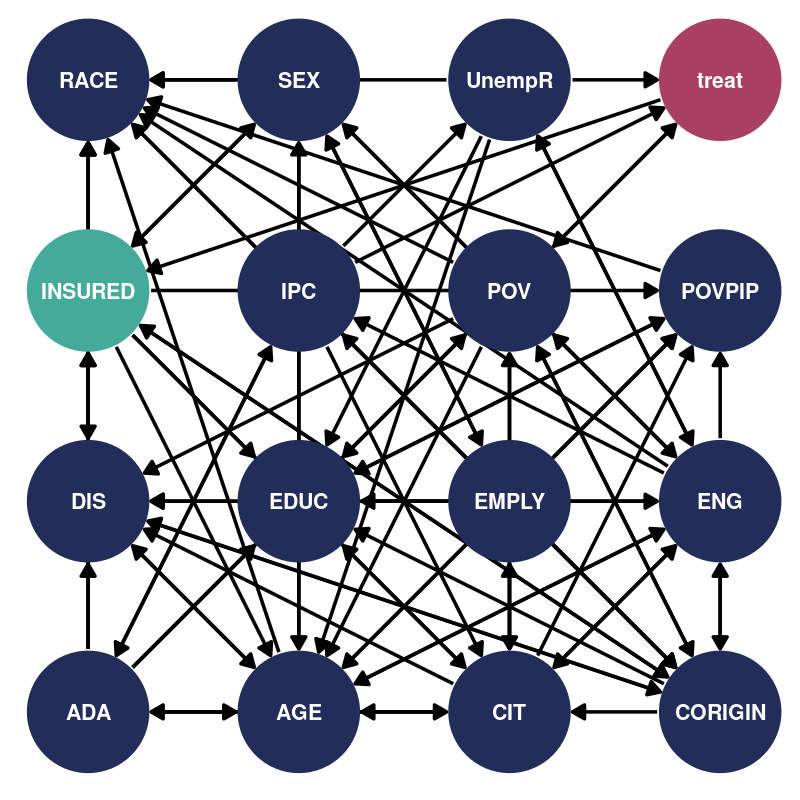
\includegraphics{~/Desktop/shadi/output/DAG1-1} \end{center}

\hypertarget{revised-casual-graph}{%
\subsubsection{Revised casual graph}\label{revised-casual-graph}}

To enhance the accuracy of the causal relationships represented in the
DAG, I carefully reviewed and manually edited the graph by removing
paths that contradicted my domain knowledge or appeared implausible
within the context. By applying these revisions, the resulting DAG,
illustrated in graph 2, aligns more closely with my expertise in the
field and provides a more trustworthy representation of the underlying
causal structure in my analysis.

\begin{center}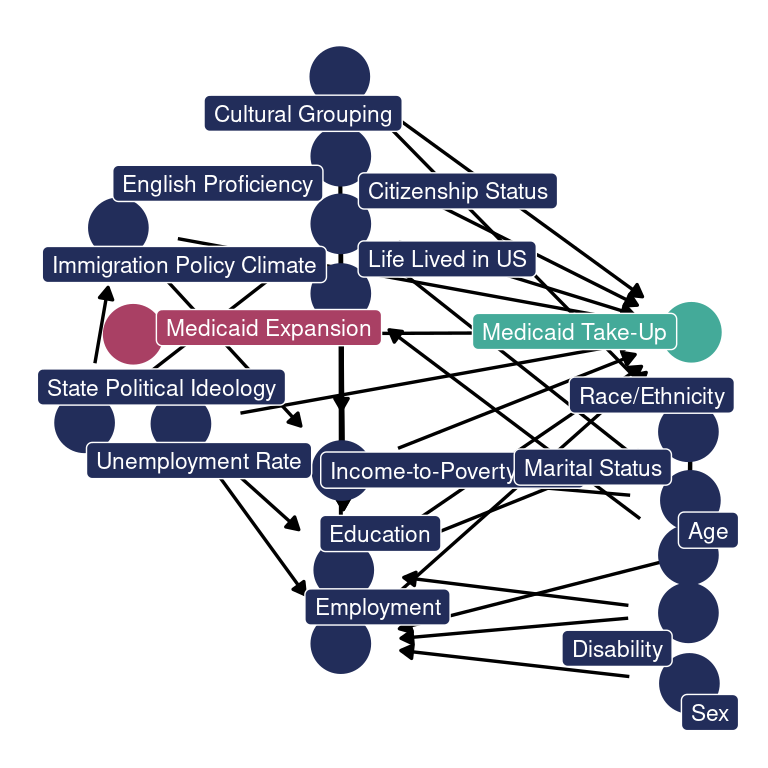
\includegraphics{~/Desktop/shadi/output/DAG2-1} \end{center}

\hypertarget{minimal-adjustment-set}{%
\subsubsection{Minimal adjustment set}\label{minimal-adjustment-set}}

The identified causal relationship between Medicaid expansion and
Medicaid take-up in the revised DAG provides compelling evidence that
changes in the treatment variable directly influence changes in the
outcome variable. This finding suggests that interventions targeting the
treatment variable, such as expanding Medicaid coverage, can potentially
have a substantial impact on improving the rate of Medicaid take-up.

by conducting backdoor analysis I identified the necessary adjustment
set, revealing that variables Citizenship Status, Immigration Policy
Climate, Unemployment Rate need to be controlled for to accurately
estimate the causal effect between Medicaid expansion and Medicaid
take-up.

\begin{Shaded}
\begin{Highlighting}[]
\FunctionTok{adjustmentSets}\NormalTok{(findag)}
\end{Highlighting}
\end{Shaded}

\begin{verbatim}
## { Citizenship Status, Immigration Policy Climate, Unemployment Rate }
## { State Political Ideology, Unemployment Rate }
\end{verbatim}

\hypertarget{simplified-causal-graph}{%
\subsubsection{Simplified causal graph}\label{simplified-causal-graph}}

To enhance the clarity and interpretability of the graph, I employed a
strategy to simplify its complexity. This involved grouping related
variables into single nodes, such as combining `education,' `income,'
and `employment' into a unified node labeled `Socioeconomic.' The
streamlined representation of the underlying relationships can be
observed in Graph 3.

\begin{center}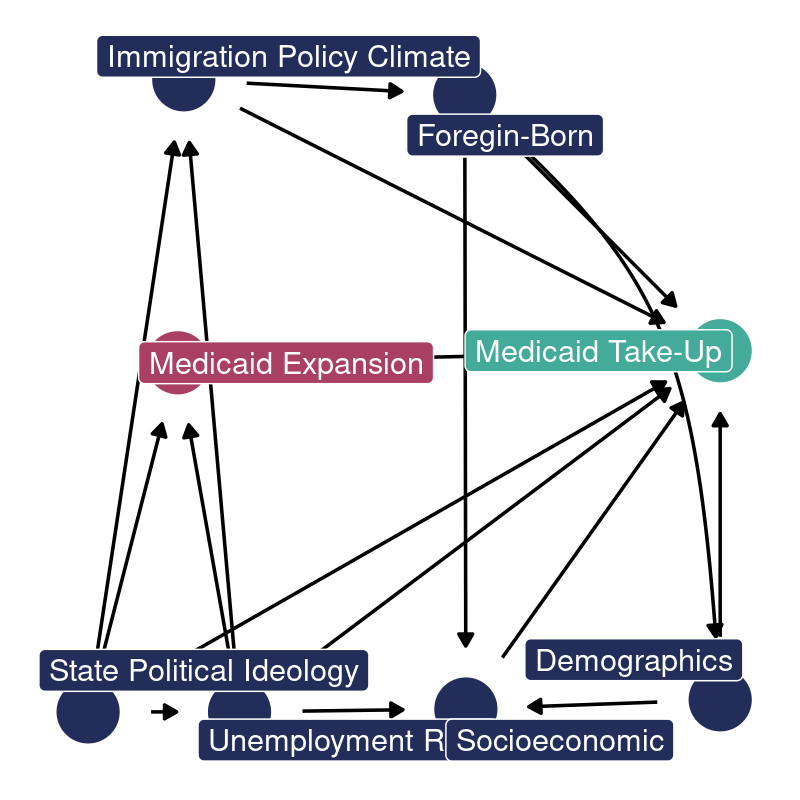
\includegraphics{~/Desktop/shadi/output/DAG3-1} \end{center}

Although utilizing causal discovery algorithms has limitations, such as
assuming the adequacy of observed variables and relying on the absence
of unobserved confounders, efforts were made to include relevant
variables in the analysis. However, it is possible that unmeasured
confounders may exist, potentially introducing biases into the
identified causal relationships. Therefore, the obtained graph may not
precisely represent the true underlying causal structure..

Due to these limitations, I do not solely rely on this graph and its
suggested adjustment set for estimating causal effects in my analysis.
Nonetheless, the DAG derived from the causal discovery approach serves
as a valuable tool for generating hypotheses and guiding the modeling
process, as well as informing the selection of control variables in my
DID approach analysis.

\hypertarget{event-study-and-parallel-trend-assumption}{%
\subsection{Event Study and Parallel Trend
Assumption}\label{event-study-and-parallel-trend-assumption}}

The main assumption of the Difference-in-Differences (DiD) methodology
relies on the presence of parallel trends before the policy
implementation.We examine the event-study estimates for uninsured rates
and Medicaid take-up to assess the impact of Medicaid expansion on
low-income individuals aged 26-64 and assess the validity of parallel
trend assumption.

\hypertarget{effect-of-the-aca-medicaid-expansions-on-uninsured-accounting-for-variation-in-treatment-timing}{%
\subsubsection{Effect of the ACA Medicaid Expansions on Uninsured:
Accounting for Variation in Treatment
Timing}\label{effect-of-the-aca-medicaid-expansions-on-uninsured-accounting-for-variation-in-treatment-timing}}

Figure 1 displays the event-study estimates for both unconditional and
conditional parallel trends for uninsured. In Panel (a), the focus is on
the effects of the expansion on uninsured without any control variables
for both US-born and foreign born individuals, while Panel (b) examines
this effects while controlling for covariates. The green line with
circles in both panels represents the foreign-borns, while the orange
line with triangle represents the US-born. For the corresponding
estimation coefficients, please refer to Table 1.

As shown in Figure 1, there are no significant pre-trend differences for
US-born individuals living in expansion states compared to non-expansion
states, as the coefficients are not significantly different from zero.
Similarly, for foreign-born individuals, the coefficients for the
interaction terms between year and the indicator for the pre-treatment
period are also small and not statistically significant, indicating no
significant pre-trend differences in the uninsured rates between
foreign-born individuals in expansion states and non-expansion states.
Moreover, when controlling for characteristics, the coefficients exhibit
minimal changes and remain small, further supporting the parallel trend
assumption. Additionally, these coefficients do not attain statistical
significance, indicating that the characteristics accounted for do not
significantly impact the parallel trends assumption.

Transitioning to the post-expansion years, we observe notable and
statistically significant declines in the overall uninsured rates for
both foreign-born and US-born individuals. The coefficients associated
with the indicator variables representing the post-expansion years are
negative and demonstrate statistical significance for both groups.
However, the change in the lead coefficients for the foreign born is
less than native suggesting that there exist disparities among native
and foreign -born.

\begin{center}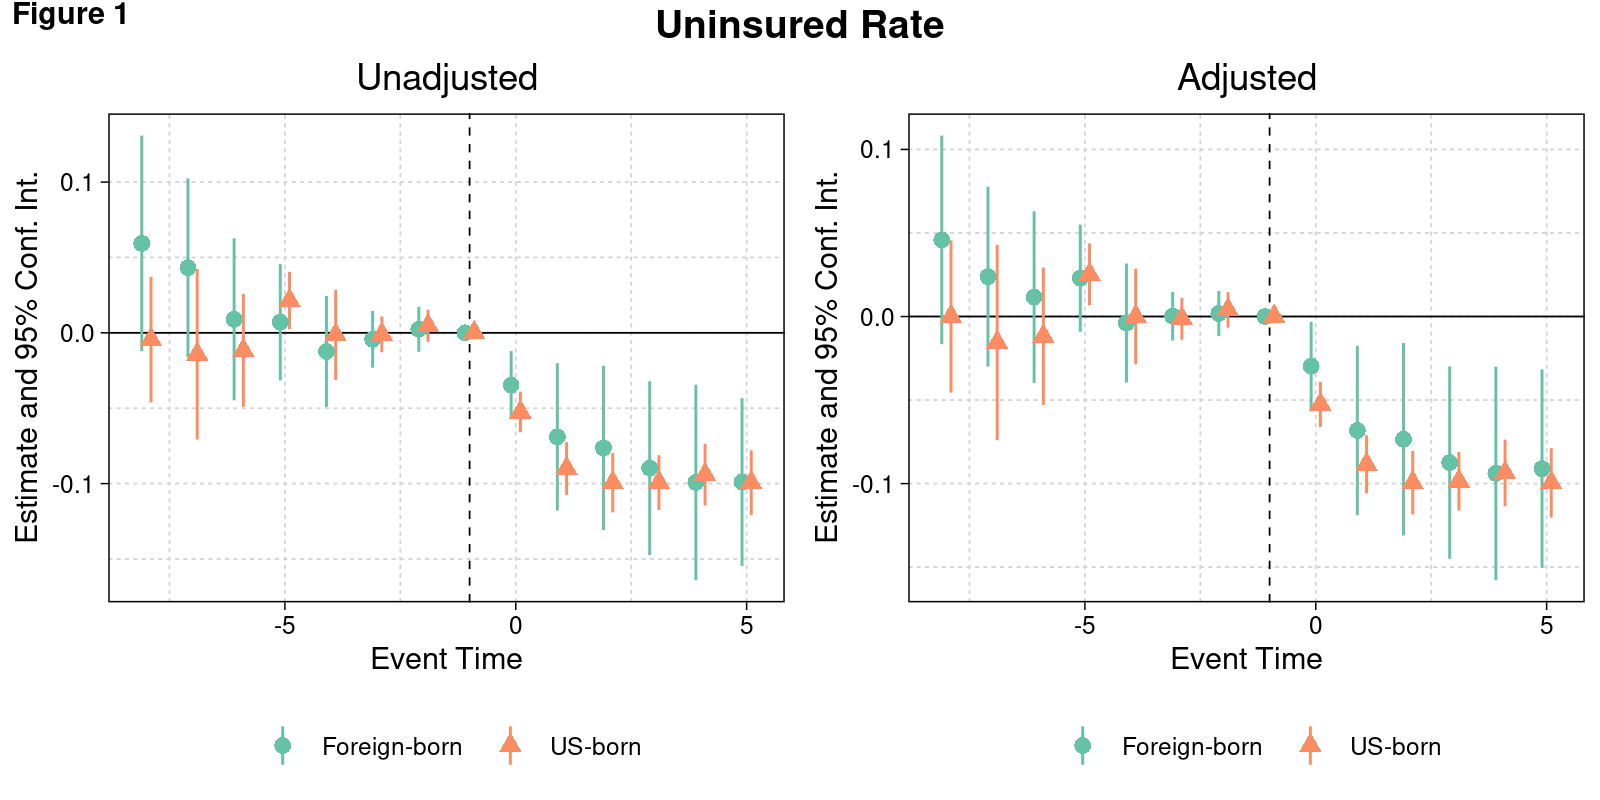
\includegraphics{~/Desktop/shadi/output/fig1-1} \end{center}

Overall, the event study presented in Figure 1 indicates significant
improvements in insurance coverage within the expansion states compared
to the non-expansion states following the implementation of Medicaid
expansion. However, the observed divergence in uninsured trends and the
smaller reduction in the uninsured rate for foreign-born individuals
highlight potential disparities in healthcare access. Table 5, presents
the result of event study.

\begin{table}[htbp]
   \caption{The Impact of Medicaid Expansion on Uninsured Rate }
   \centering
   \small
   \renewcommand*{\arraystretch}{0.5}
   \begin{tabular}{lcccc}
      \tabularnewline \midrule \midrule
       & \multicolumn{2}{c}{US-born} & \multicolumn{2}{c}{Foreign-Born} \\ \cmidrule(lr){2-3} \cmidrule(lr){4-5}
      Variables             & (1)            & (2)                    & (3)            & (4)\\  
      \midrule 
      expansion year $=$ -8 & -0.005         & $3.95\times 10^{-5}$   & 0.059$^{*}$    & 0.046\\   
                            & (0.021)        & (0.023)                & (0.030)        & (0.028)\\   
      expansion year $=$ -7 & -0.014         & -0.015                 & 0.043          & 0.024\\   
                            & (0.025)        & (0.026)                & (0.028)        & (0.025)\\   
      expansion year $=$ -6 & -0.012         & -0.012                 & 0.009          & 0.012\\   
                            & (0.019)        & (0.021)                & (0.026)        & (0.026)\\   
      expansion year $=$ -5 & 0.021$^{*}$    & 0.025$^{**}$           & 0.007          & 0.023\\   
                            & (0.011)        & (0.011)                & (0.018)        & (0.016)\\   
      expansion year $=$ -4 & -0.001         & $-2.61\times 10^{-5}$  & -0.012         & -0.004\\   
                            & (0.017)        & (0.017)                & (0.016)        & (0.017)\\   
      expansion year $=$ -3 & -0.001         & -0.001                 & -0.004         & 0.0002\\   
                            & (0.004)        & (0.005)                & (0.010)        & (0.009)\\   
      expansion year $=$ -2 & 0.005          & 0.004                  & 0.002          & 0.002\\   
                            & (0.003)        & (0.004)                & (0.008)        & (0.007)\\   
      expansion year $=$ 0  & -0.052$^{***}$ & -0.053$^{***}$         & -0.035$^{***}$ & -0.030$^{**}$\\   
                            & (0.005)        & (0.005)                & (0.008)        & (0.011)\\   
      expansion year $=$ 1  & -0.090$^{***}$ & -0.088$^{***}$         & -0.069$^{**}$  & -0.068$^{**}$\\   
                            & (0.008)        & (0.008)                & (0.024)        & (0.024)\\   
      expansion year $=$ 2  & -0.100$^{***}$ & -0.100$^{***}$         & -0.076$^{**}$  & -0.073$^{**}$\\   
                            & (0.009)        & (0.009)                & (0.026)        & (0.027)\\   
      expansion year $=$ 3  & -0.099$^{***}$ & -0.099$^{***}$         & -0.090$^{**}$  & -0.087$^{**}$\\   
                            & (0.008)        & (0.008)                & (0.028)        & (0.028)\\   
      expansion year $=$ 4  & -0.094$^{***}$ & -0.094$^{***}$         & -0.099$^{**}$  & -0.094$^{**}$\\   
                            & (0.009)        & (0.009)                & (0.030)        & (0.030)\\   
      expansion year $=$ 5  & -0.100$^{***}$ & -0.100$^{***}$         & -0.099$^{***}$ & -0.091$^{**}$\\   
                            & (0.009)        & (0.009)                & (0.026)        & (0.027)\\   
      State FE              & yes            & yes                    & yes            & yes\\  
      Year FE               & yes            & yes                    & yes            & yes\\  
      Controls              &                & yes                    &                & yes\\  
      Observations          & 1,585,639      & 1,585,639              & 389,955        & 389,955\\  
      R$^2$                 & 0.05930        & 0.11985                & 0.08577        & 0.21524\\  
      Within R$^2$          & 0.00286        & 0.06704                & 0.00172        & 0.14309\\  
      \midrule \midrule
      \multicolumn{5}{l}{\emph{Clustered (State \& Year) standard-errors in parentheses}}\\
      \multicolumn{5}{l}{\emph{Signif. Codes: ***: 0.01, **: 0.05, *: 0.1}}\\
   \end{tabular}
\end{table}

\hypertarget{effect-of-the-aca-medicaid-expansions-on-medicaid-coverage-accounting-for-variation-in-treatment-timing}{%
\subsubsection{Effect of the ACA Medicaid Expansions on Medicaid
Coverage: Accounting for Variation in Treatment
Timing}\label{effect-of-the-aca-medicaid-expansions-on-medicaid-coverage-accounting-for-variation-in-treatment-timing}}

Figure 2 and Table 2 present the event-study estimates for the
unconditional and conditional parallel trends concerning Medicaid
take-up. According to the data presented in Figure 2,prior to the
implementation of Medicaid expansion, there is no significant pre-trend
difference in Medicaid take-up between expansion and non-expansion
states for both low-income US-born and foreign-born individuals aged
26-64.

For the US-born sub-sample, Model 2 includes control variables, while
Model 1 serves as a baseline model. The coefficients for the interaction
terms between year and the indicator for the pre-treatment period were
generally small and statistically insignificant in both models. This
suggests that there is no significant pre-trend difference in uninsured
rates between expansion and non-expansion states for US-born
individuals.

\begin{center}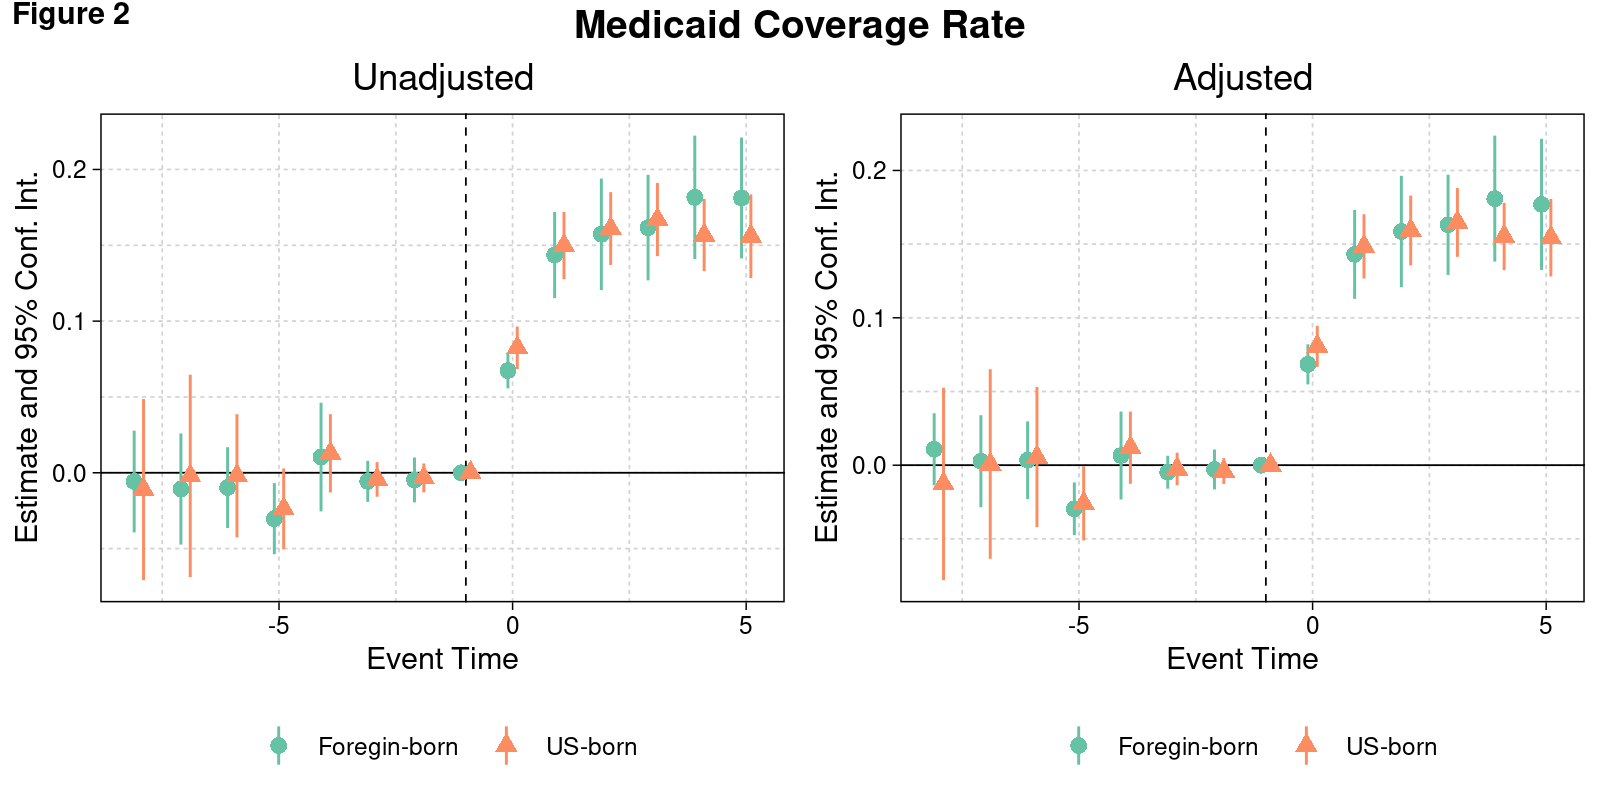
\includegraphics{~/Desktop/shadi/output/fig2-1} \end{center}

Similarly, for the foreign-born sub-sample,As shown in the table 6.
model 4 includes control variables, while model 3 serves as a baseline
model. The coefficients for the interaction terms were also small and
statistically insignificant in both models, suggesting no significant
pre-trend difference in uninsured rates between expansion and
non-expansion states for foreign-born individuals.

Furthermore, the coefficients for the interaction terms representing the
post-treatment periods (years 0 to 5 after the implementation of
Medicaid expansion) were positive and statistically significant in all
models, indicating an increase in medicaid coverage for both US-born and
foreign-born individuals in expansion states compared to non-expansion
states during those years. Hpwever, a notable pattern emerges regarding
the Medicaid take-up between foreign-born and US-born individuals
following the expansion. Initially, during the first three years after
the expansion, the Medicaid take-up for foreign-born individuals was
similar to that of US-born individuals; but, from year 4 onwardsa we
observe that the take-up rate among foreign-born individuals increased.
This suggests that over time, foreign-born individuals were able to
overcome some of the barriers and obstacles they initially encountered,
leading to a higher participation in Medicaid. It is likely that various
factors contributed to this trend. Changes in immigration policies,
targeted outreach efforts aimed at foreign-born populations, or the
implementation of programs specifically designed to enhance healthcare
access for immigrants could have played a role in facilitating the
increased participation among foreign-born individuals. Further
investigation into the specific policies and initiatives implemented
during this period would provide a deeper understanding of the factors
influencing the changing Medicaid take-up rates among foreign-born
individuals.

\begin{longtable}[]{@{}
  >{\centering\arraybackslash}p{(\columnwidth - 0\tabcolsep) * \real{1.0000}}@{}}
\toprule\noalign{}
\endhead
\bottomrule\noalign{}
\endlastfoot
\textbf{NOTE:} \\
It is surprising to me see a higher Medicaid take-up rate for
foreign-born individuals during the fourth and fifth years after
expansion, since it aligns with the years 2018 and 2019 when stricter
immigration policies were implemented under the Trump administration. \\
\end{longtable}

\FloatBarrier

\begin{table}[htbp]
   \caption{The Impact of Medicaid Expansion on Medicaid Coverage }
   \centering
   \small
   \begin{adjustbox}{width = 0.6\textwidth, center}
      \renewcommand*{\arraystretch}{0.5}
      \begin{tabular}{lcccc}
         \tabularnewline \midrule \midrule
          & \multicolumn{2}{c}{US-born} & \multicolumn{2}{c}{Foreign-Born} \\ \cmidrule(lr){2-3} \cmidrule(lr){4-5}
         Variables             & (1)           & (2)           & (3)            & (4)\\  
         \midrule 
         expansion year $=$ -8 & -0.011        & -0.013        & -0.006         & 0.011\\   
                               & (0.029)       & (0.031)       & (0.009)        & (0.008)\\   
         expansion year $=$ -7 & -0.002        & 0.0008        & -0.011         & 0.003\\   
                               & (0.031)       & (0.031)       & (0.013)        & (0.011)\\   
         expansion year $=$ -6 & -0.002        & 0.005         & -0.010         & 0.003\\   
                               & (0.021)       & (0.024)       & (0.011)        & (0.011)\\   
         expansion year $=$ -5 & -0.024        & -0.026$^{*}$  & -0.030$^{***}$ & -0.030$^{***}$\\   
                               & (0.014)       & (0.013)       & (0.008)        & (0.007)\\   
         expansion year $=$ -4 & 0.013         & 0.012         & 0.010          & 0.007\\   
                               & (0.015)       & (0.015)       & (0.017)        & (0.015)\\   
         expansion year $=$ -3 & -0.004        & -0.003        & -0.006         & -0.005\\   
                               & (0.003)       & (0.003)       & (0.006)        & (0.006)\\   
         expansion year $=$ -2 & -0.003        & -0.004        & -0.005         & -0.003\\   
                               & (0.004)       & (0.004)       & (0.007)        & (0.007)\\   
         expansion year $=$ 0  & 0.082$^{***}$ & 0.081$^{***}$ & 0.067$^{***}$  & 0.068$^{***}$\\   
                               & (0.004)       & (0.005)       & (0.002)        & (0.004)\\   
         expansion year $=$ 1  & 0.150$^{***}$ & 0.148$^{***}$ & 0.144$^{***}$  & 0.143$^{***}$\\   
                               & (0.011)       & (0.011)       & (0.013)        & (0.014)\\   
         expansion year $=$ 2  & 0.161$^{***}$ & 0.159$^{***}$ & 0.157$^{***}$  & 0.159$^{***}$\\   
                               & (0.011)       & (0.012)       & (0.017)        & (0.018)\\   
         expansion year $=$ 3  & 0.167$^{***}$ & 0.165$^{***}$ & 0.162$^{***}$  & 0.163$^{***}$\\   
                               & (0.011)       & (0.012)       & (0.017)        & (0.016)\\   
         expansion year $=$ 4  & 0.157$^{***}$ & 0.155$^{***}$ & 0.182$^{***}$  & 0.181$^{***}$\\   
                               & (0.010)       & (0.010)       & (0.018)        & (0.020)\\   
         expansion year $=$ 5  & 0.156$^{***}$ & 0.154$^{***}$ & 0.181$^{***}$  & 0.177$^{***}$\\   
                               & (0.011)       & (0.011)       & (0.017)        & (0.020)\\   
         State FE              & yes           & yes           & yes            & yes\\  
         Year FE               & yes           & yes           & yes            & yes\\  
         Controls              &               & yes           &                & yes\\  
         Observations          & 1,585,639     & 1,585,639     & 389,955        & 389,955\\  
         R$^2$                 & 0.06514       & 0.18789       & 0.10655        & 0.18046\\  
         Within R$^2$          & 0.00628       & 0.13676       & 0.00837        & 0.09041\\  
         \midrule \midrule
         \multicolumn{5}{l}{\emph{Clustered (State \& Year) standard-errors in parentheses}}\\
         \multicolumn{5}{l}{\emph{Signif. Codes: ***: 0.01, **: 0.05, *: 0.1}}\\
      \end{tabular}
   \end{adjustbox}
\end{table}

These findings demonstrate the effectiveness of Medicaid expansion in
improving access to healthcare, especially among foreign-born
individuals. The absence of significant pre-trend differences and the
subsequent increase in Medicaid take-up rates following the expansion
highlight the positive impact of the expansion in reducing the uninsured
population and promoting healthcare coverage for both US-born and
foreign-born individuals in expansion states compared to non-expansion
states.These findings demonstrate the effectiveness of Medicaid
expansion in improving access to healthcare, especially among
foreign-born individuals. The absence of significant pre-trend
differences and the subsequent increase in Medicaid take-up rates
following the expansion highlight the positive impact of the expansion
in reducing the uninsured population and promoting healthcare coverage
for both US-born and foreign-born individuals in expansion states
compared to non-expansion states.

\hypertarget{difference-in-differences-model-results}{%
\subsection{Difference-in-Differences Model
Results}\label{difference-in-differences-model-results}}

We first examine the effect of Medicaid expansion on the uninsured rate.
Table 7, presents the primary findings of the difference-in-differences
(DD) analysis, which includes sample weights and adjusts for covariates.
The first seven columns display estimates from the fixed effect linear
probability model, while the second seven columns show results from the
fixed effect logit model. Each specification controls for state and year
fixed effects. Column 2 includes controls for state political ideology
and state unemployment rate, which were identified as the minimal
adjustment set based on the result of the directed acyclic graph (DAG)
causal discovery. Column 3 additionally controls for region-by-year
fixed effects, while column 4 controls for state-specific linear time
trends. The full model with all the control variables added is presented
in columns 5-7, where column 6 includes region-by-year fixed effects and
column 7 includes state-specific linear time trends.

Among FE OLS models, the estimated effect of Medicaid expansion on the
uninsured ranges from -0.044 to -0.092 across different specifications
(columns 1 to 7). These estimates suggest that Medicaid expansion
reduces the probability of being uninsured by approximately 4.4\% to
9.2\%. Among FE LOGIT model, the estimated effect ranges from -0.333 to
-0.629 across different specifications (columns 8 to 14). Since the FE
LOGIT model estimates the effect in terms of odds ratios, the estimates
suggest that Medicaid expansion reduces the odds of being uninsured by
approximately 33.3\% to 62.9\%. Furthermore, the models indicate that
being foreign-born is associated with an increase in the probability of
being uninsured in the FE OLS model, while it increases the odds of
being uninsured in the FE LOGIT model. Both models show a negative and
statistically significant interaction term, indicating that the effect
of Medicaid expansion on the uninsured rate is smaller for foreign-born
individuals compared to the US-born population. To assess the goodness
of fit of the models, we consider the adjusted R-squared for the FE OLS
model and the Pseudo R-squared and BIC for both models. The FE OLS model
in column 7 exhibits the highest adjusted R-squared value of 0.17830 and
the lowest BIC value of 2,206,836.9. For the FE LOGIT model, column 14
has the highest Pseudo R-squared value of 0.15066 and the lowest BIC
value of 240,927,239.1.These measures help evaluate the fit of the
models to the data, with higher adjusted R-squared and Pseudo R-squared
values indicating better fit, and lower BIC values suggesting better
model performance.

\begin{longtable}[]{@{}
  >{\raggedright\arraybackslash}p{(\columnwidth - 0\tabcolsep) * \real{1.0000}}@{}}
\toprule\noalign{}
\endhead
\bottomrule\noalign{}
\endlastfoot
\textbf{\emph{To DO Shadi:}} \\
The BIC and Pseudo R-squared are off check why is that. Given that LOGIT
is prefered over PLM should I choose col 14 as my prefered model? should
I add or remove any specificaiton? \\
\end{longtable}

\blandscape

\begin{table}[htbp]
   \centering
   \begin{adjustbox}{width = 1.5\textwidth, center}
      \begin{threeparttable}[b]
         \caption{The Effect of Medicaid Expansion on Uninsured Rate (Difference-in-Differences Estimation)}
         \renewcommand*{\arraystretch}{1}
         \begin{tabular}{lcccccccccccccc}
            \tabularnewline \midrule \midrule
             & \multicolumn{7}{c}{FE OLS} & \multicolumn{7}{c}{FE LOGIT} \\ \cmidrule(lr){2-8} \cmidrule(lr){9-15}
                                                      & (1)            & (2)            & (3)            & (4)            & (5)            & (6)            & (7)            & (8)            & (9)            & (10)           & (11)           & (12)           & (13)           & (14)\\  
            \midrule 
            Medicaid Expansion                        & -0.075$^{***}$ & -0.071$^{***}$ & -0.085$^{***}$ & -0.044$^{***}$ & -0.081$^{***}$ & -0.092$^{***}$ & -0.053$^{***}$ & -0.568$^{***}$ & -0.549$^{***}$ & -0.572$^{***}$ & -0.333$^{***}$ & -0.612$^{***}$ & -0.629$^{***}$ & -0.384$^{***}$\\   
                                                      & (0.002)        & (0.002)        & (0.002)        & (0.003)        & (0.002)        & (0.002)        & (0.003)        & (0.009)        & (0.009)        & (0.012)        & (0.015)        & (0.009)        & (0.012)        & (0.015)\\   
            Foreign-Born                              & 0.244$^{***}$  & 0.243$^{***}$  & 0.243$^{***}$  & 0.244$^{***}$  & -0.229$^{***}$ & 2.27           & -0.064$^{***}$ & 1.03$^{***}$   & 1.02$^{***}$   & 1.02$^{***}$   & 1.03$^{***}$   & -0.389$^{***}$ & -0.406$^{***}$ & 9.60$^{***}$\\   
                                                      & (0.001)        & (0.001)        & (0.001)        & (0.001)        & (0.008)        & (2.17)         & (0.015)        & (0.006)        & (0.006)        & (0.006)        & (0.006)        & (0.083)        & (0.083)        & (0.228)\\   
            Medicaid Expansion $\times$ Foreign-Born  & -0.031$^{***}$ & -0.029$^{***}$ & -0.028$^{***}$ & -0.031$^{***}$ & 0.0004         & 0.004$^{*}$    & 0.0009         & 0.170$^{***}$  & 0.186$^{***}$  & 0.199$^{***}$  & 0.180$^{***}$  & 0.222$^{***}$  & 0.253$^{***}$  & 0.240$^{***}$\\   
                                                      & (0.002)        & (0.002)        & (0.002)        & (0.002)        & (0.002)        & (0.002)        & (0.002)        & (0.011)        & (0.011)        & (0.011)        & (0.011)        & (0.011)        & (0.012)        & (0.012)\\   
            State Unemployment Rate                   &                & 0.004$^{***}$  & 0.005$^{***}$  & 0.002$^{**}$   &                &                &                &                & 0.021$^{***}$  & 0.023$^{***}$  & 0.010$^{**}$   &                &                &   \\   
                                                      &                & (0.0006)       & (0.0007)       & (0.0010)       &                &                &                &                & (0.003)        & (0.003)        & (0.005)        &                &                &   \\   
            State Political Ideology                  &                & -0.011         & 0.015$^{*}$    & -0.044$^{***}$ &                &                &                &                & -0.162$^{***}$ & -0.026         & -0.271$^{***}$ &                &                &   \\   
                                                      &                & (0.008)        & (0.009)        & (0.012)        &                &                &                &                & (0.044)        & (0.047)        & (0.062)        &                &                &   \\   
            \midrule 
            Controls                                  &                &                &                &                & yes            & yes            & yes            &                &                &                &                & yes            & yes            & yes\\  
            State FE                                  & yes            & yes            & yes            & yes            & yes            & yes            & yes            & yes            & yes            & yes            & yes            & yes            & yes            & yes\\  
            Year FE                                   & yes            & yes            & yes            & yes            & yes            & yes            & yes            & yes            & yes            & yes            & yes            & yes            & yes            & yes\\  
            Region-Year FE                            &                &                & yes            &                &                & yes            &                &                &                & yes            &                &                & yes            & \\  
            State-Specific Linear Time Trends         &                &                &                & yes            &                &                & yes            &                &                &                & yes            &                &                & yes\\  
            \midrule 
            Convergence                               &TRUE            & TRUE           & TRUE           & TRUE           & TRUE           & TRUE           & TRUE           & TRUE           & TRUE           & TRUE           & TRUE           & TRUE           & TRUE           & FALSE\\  
            Standard-Errors & \multicolumn{14}{c}{Heteroskedasticity-robust} \\ 
            Observations                              & 1,975,594      & 1,975,594      & 1,975,594      & 1,975,594      & 1,975,594      & 1,975,594      & 1,975,594      & 1,975,594      & 1,975,594      & 1,975,594      & 1,975,594      & 1,975,594      & 1,975,594      & 1,975,594\\  
            R$^2$                                     & 0.10174        & 0.10180        & 0.10226        & 0.10282        & 0.17730        & 0.17502        & 0.17836        &                &                &                &                &                &                & \\  
            Adjusted R$^2$                            & 0.10172        & 0.10177        & 0.10222        & 0.10278        & 0.17726        & 0.17496        & 0.17830        &                &                &                &                &                &                & \\  
            Pseudo R$^2$                              & 0.99202        & 0.99202        & 0.99203        & 0.99203        & 0.99257        & 0.99256        & 0.99258        & 0.08279        & -105.71        & -105.66        & 0.08385        & -97.947        & -97.888        & 0.15066\\  
            AIC                                       & 2,370,925.9    & 2,370,831.8    & 2,370,046.4    & 2,368,702.0    & 2,207,430.9    & 2,211,565.1    & 2,205,087.4    & 260,176,660.9  & 260,157,000.2  & 260,034,591.5  & 259,874,375.8  & 241,235,358.9  & 241,091,334.3  & 240,925,477.2\\  
            BIC                                       & 2,371,638.2    & 2,371,581.6    & 2,371,233.5    & 2,370,014.1    & 2,208,630.5    & 2,213,214.6    & 2,206,836.9    & 260,177,373.2  & 260,157,750.0  & 260,035,778.6  & 259,875,687.9  & 241,236,546.0  & 241,092,958.8  & 240,927,239.1\\  
            \midrule \midrule
            \multicolumn{15}{l}{\emph{Heteroskedasticity-robust standard-errors in parentheses}}\\
            \multicolumn{15}{l}{\emph{Signif. Codes: ***: 0.01, **: 0.05, *: 0.1}}\\
         \end{tabular}
      \end{threeparttable}
   \end{adjustbox}
\end{table}

\elandscape

We then shift our focus to analyzing the impact of Medicaid expansion on
Medicaid coverage using Table 8. This table follows a similar structure
to Table 7, with the FE Linear probability model estimates in the first
seven columns and the FE logit model estimates in the second seven
columns. Both models include state and year fixed effects to account for
potential confounding factors.In the FE OLS model, the estimated effect
of Medicaid expansion on the Medicaid coverage rate ranges from 0.085 to
0.148 across different specifications (columns 1 to 7). These estimates
suggest that Medicaid expansion increases the probability of individuals
being covered by Medicaid by approximately 8.5\% to 14.8\%. Similarly,
in the FE logit model, the estimated effect ranges from 0.305 to 0.660
(columns 8 to 14), indicating that Medicaid expansion increases the odds
of being covered by Medicaid. We also examine the impact of foreign-born
status on the Medicaid coverage rate. In the FE OLS model, being
foreign-born is associated with a decreased probability in having
Medicaid coverage, while in the FE logit model, it decreases the odds of
being covered by Medicaid.Moreover, the interaction term between
Medicaid expansion and foreign-born status shows a significant
relationship in both models. However, the magnitude and direction of
this interaction term vary across different models and specifications.
In columns 5, 6, and 7 of the table, negative coefficients are observed
for the interaction term between Medicaid expansion and foreign-born
status. This indicates that in those specific model specifications, the
effect of Medicaid expansion on the Medicaid coverage rate is smaller
for foreign-born individuals compared to the US-born population. For
example, in column 1 and 5, the coefficient of the interaction term is
positive but small in magnitude, suggesting that Medicaid expansion has
a small positive effect on the probability of foreign-born individuals
being covered compared to US-born individuals. However, as additional
covariates are included in the model, the coefficient becomes negative
in columns 6 and 7, indicating a smaller effect of Medicaid expansion
for foreign-born individuals. In the FE logit model specifications, the
odds of being covered by Medicaid due to Medicaid expansion are positive
for foreign-born individuals but decrease as additional covariates are
included. In our preferred model (column 14), the odds are estimated to
be 16\%, indicating a substantial increase in the likelihood of Medicaid
coverage for foreign-born individuals due to Medicaid expansion.

Similar to Table 7, we assess the goodness of fit using R-squared,
adjusted R-squared, pseudo R-squared, AIC, and BIC. In the FE OLS model,
the R-squared ranges from 0.08522 to 0.19483, and the adjusted R-squared
ranges from 0.08520 to 0.19477 (columns 1 to 7). For the FE logit model,
the pseudo R-squared ranges from -104.05 to 0.15944 (columns 8 to 14).
Lower AIC and BIC values indicate better model performance. Based on
these measures, the preferred model specifications in Table 8 may be
column 7 in the FE OLS model and column 14 in the FE logit model. These
specifications exhibit higher R-squared, adjusted R-squared, and pseudo
R-squared values, as well as lower AIC and BIC values, indicating better
fit and performance.

\blandscape

\begin{table}[htbp]
   \centering
   \large
   \begin{adjustbox}{width = 1.5\textwidth, center}
      \begin{threeparttable}[b]
         \caption{The Effect of Medicaid Expansion on Medicaid Covergare Rate (Difference-in-Differences Estimation)}
         \renewcommand*{\arraystretch}{1}
         \begin{tabular}{lcccccccccccccc}
            \tabularnewline \midrule \midrule
             & \multicolumn{7}{c}{FE OLS} & \multicolumn{7}{c}{FE LOGIT} \\ \cmidrule(lr){2-8} \cmidrule(lr){9-15}
                                                      & (1)            & (2)            & (3)            & (4)            & (5)            & (6)            & (7)            & (8)            & (9)            & (10)           & (11)           & (12)          & (13)          & (14)\\  
            \midrule 
            Medicaid Expansion                        & 0.136$^{***}$  & 0.134$^{***}$  & 0.144$^{***}$  & 0.085$^{***}$  & 0.140$^{***}$  & 0.148$^{***}$  & 0.092$^{***}$  & 0.498$^{***}$  & 0.493$^{***}$  & 0.554$^{***}$  & 0.305$^{***}$  & 0.591$^{***}$ & 0.660$^{***}$ & 0.390$^{***}$\\   
                                                      & (0.002)        & (0.002)        & (0.002)        & (0.003)        & (0.002)        & (0.002)        & (0.003)        & (0.008)        & (0.009)        & (0.011)        & (0.013)        & (0.009)       & (0.011)       & (0.013)\\   
            Foreign-Born                              & -0.158$^{***}$ & -0.158$^{***}$ & -0.157$^{***}$ & -0.159$^{***}$ & 0.086$^{***}$  & -0.634         & -0.002         & -0.862$^{***}$ & -0.863$^{***}$ & -0.859$^{***}$ & -0.869$^{***}$ & -0.034        & -0.021        & -0.035\\   
                                                      & (0.001)        & (0.001)        & (0.001)        & (0.001)        & (0.007)        & (2.47)         & (0.015)        & (0.007)        & (0.007)        & (0.007)        & (0.007)        & (0.082)       & (0.082)       & (0.082)\\   
            Medicaid Expansion $\times$ Foreign-Born  & 0.007$^{***}$  & 0.007$^{***}$  & 0.005$^{**}$   & 0.009$^{***}$  & -0.012$^{***}$ & -0.016$^{***}$ & -0.012$^{***}$ & 0.239$^{***}$  & 0.241$^{***}$  & 0.233$^{***}$  & 0.256$^{***}$  & 0.151$^{***}$ & 0.136$^{***}$ & 0.163$^{***}$\\   
                                                      & (0.002)        & (0.002)        & (0.002)        & (0.002)        & (0.002)        & (0.002)        & (0.002)        & (0.010)        & (0.011)        & (0.011)        & (0.011)        & (0.011)       & (0.011)       & (0.012)\\   
            State Unemployment Rate                   &                & -0.003$^{***}$ & -0.003$^{***}$ & -0.003$^{***}$ &                &                &                &                & -0.011$^{***}$ & -0.014$^{***}$ & -0.015$^{***}$ &               &               &   \\   
                                                      &                & (0.0006)       & (0.0007)       & (0.0010)       &                &                &                &                & (0.003)        & (0.003)        & (0.005)        &               &               &   \\   
            State Political Ideology                  &                & -0.035$^{***}$ & -0.074$^{***}$ & 0.025$^{**}$   &                &                &                &                & -0.201$^{***}$ & -0.368$^{***}$ & 0.082          &               &               &   \\   
                                                      &                & (0.009)        & (0.009)        & (0.012)        &                &                &                &                & (0.040)        & (0.043)        & (0.056)        &               &               &   \\   
            \midrule 
            Controls                                  &                &                &                &                & yes            & yes            & yes            &                &                &                &                & yes           & yes           & yes\\  
            State FE                                  & yes            & yes            & yes            & yes            & yes            & yes            & yes            & yes            & yes            & yes            & yes            & yes           & yes           & yes\\  
            Year FE                                   & yes            & yes            & yes            & yes            & yes            & yes            & yes            & yes            & yes            & yes            & yes            & yes           & yes           & yes\\  
            Region-Year FE                            &                &                & yes            &                &                & yes            &                &                &                & yes            &                &               & yes           & \\  
            State-Specific Linear Time Trends         &                &                &                & yes            &                &                & yes            &                &                &                & yes            &               &               & yes\\  
            \midrule 
            Convergence                               &TRUE            & TRUE           & TRUE           & TRUE           & TRUE           & TRUE           & TRUE           & TRUE           & TRUE           & TRUE           & TRUE           & TRUE          & TRUE          & TRUE\\  
            Standard-Errors & \multicolumn{14}{c}{Heteroskedasticity-robust} \\ 
            Observations                              & 1,975,594      & 1,975,594      & 1,975,594      & 1,975,594      & 1,975,594      & 1,975,594      & 1,975,594      & 1,975,594      & 1,975,594      & 1,975,594      & 1,975,594      & 1,975,594     & 1,975,594     & 1,975,594\\  
            R$^2$                                     & 0.08522        & 0.08525        & 0.08589        & 0.08677        & 0.19330        & 0.19379        & 0.19483        &                &                &                &                &               &               & \\  
            Adjusted R$^2$                            & 0.08520        & 0.08522        & 0.08585        & 0.08672        & 0.19326        & 0.19374        & 0.19477        &                &                &                &                &               &               & \\  
            Pseudo R$^2$                              & 0.99160        & 0.99160        & 0.99161        & 0.99161        & 0.99240        & 0.99240        & 0.99241        & 0.06642        & -104.05        & -104.00        & 0.06752        & -93.720       & -93.669       & 0.15944\\  
            AIC                                       & 2,625,715.2    & 2,625,657.5    & 2,624,691.9    & 2,622,755.7    & 2,377,784.4    & 2,376,890.4    & 2,374,515.4    & 278,454,421.5  & 278,448,734.1  & 278,318,864.0  & 278,125,737.5  & 251,077,717.7 & 250,941,054.9 & 250,708,901.3\\  
            BIC                                       & 2,626,427.5    & 2,626,407.3    & 2,625,879.1    & 2,624,067.8    & 2,378,984.1    & 2,378,539.9    & 2,376,264.9    & 278,455,133.8  & 278,449,483.9  & 278,320,051.2  & 278,127,049.6  & 251,078,904.8 & 250,942,679.5 & 250,710,650.8\\  
            \midrule \midrule
            \multicolumn{15}{l}{\emph{Heteroskedasticity-robust standard-errors in parentheses}}\\
            \multicolumn{15}{l}{\emph{Signif. Codes: ***: 0.01, **: 0.05, *: 0.1}}\\
         \end{tabular}
      \end{threeparttable}
   \end{adjustbox}
\end{table}

\elandscape

\hypertarget{sensitivity-and-robustness-check}{%
\subsection{Sensitivity and Robustness
Check}\label{sensitivity-and-robustness-check}}

\hypertarget{heterogeneous-treatment-effects-sun-abraham-2020}{%
\subsubsection{Heterogeneous Treatment Effects: Sun \& Abraham
(2020)}\label{heterogeneous-treatment-effects-sun-abraham-2020}}

Since 2018, there has been a growing body of literature examining the
validity of staggered Difference-in-Differences (DID) models and event
study designs. Noteworthy studies in this field include Goodman-Bacon
(2018), Callaway and Sant'anna (2020), de Chaisemartin and
D'aualtfoeuille (2020), Deshpande and Li (2019), Imai and Kim (2021),
and Baker et al.~(2021). Sun and Abraham (2021) highlight the challenges
that can arise when different treatment cohorts exhibit varying
treatment effects over time.

To address these concerns and assess the sensitivity of our event study
estimates to heterogeneous treatment effects, we adopt the
interaction-weighted (IW) event study estimator proposed by Sun and
Abraham (2021). This estimator is robust to variations in treatment
effects across cohorts. We estimate event study coefficients separately
for each group and outcome, and then aggregate these coefficients using
the fraction of the treated sample in each group as weights for the
relevant period. Importantly, the results of this analysis align with
our main findings.

We find no evidence of differential pre-trends, leading us to conclude
that our results are robust and not unduly influenced by variations in
treatment profiles across different cohorts.

\begin{center}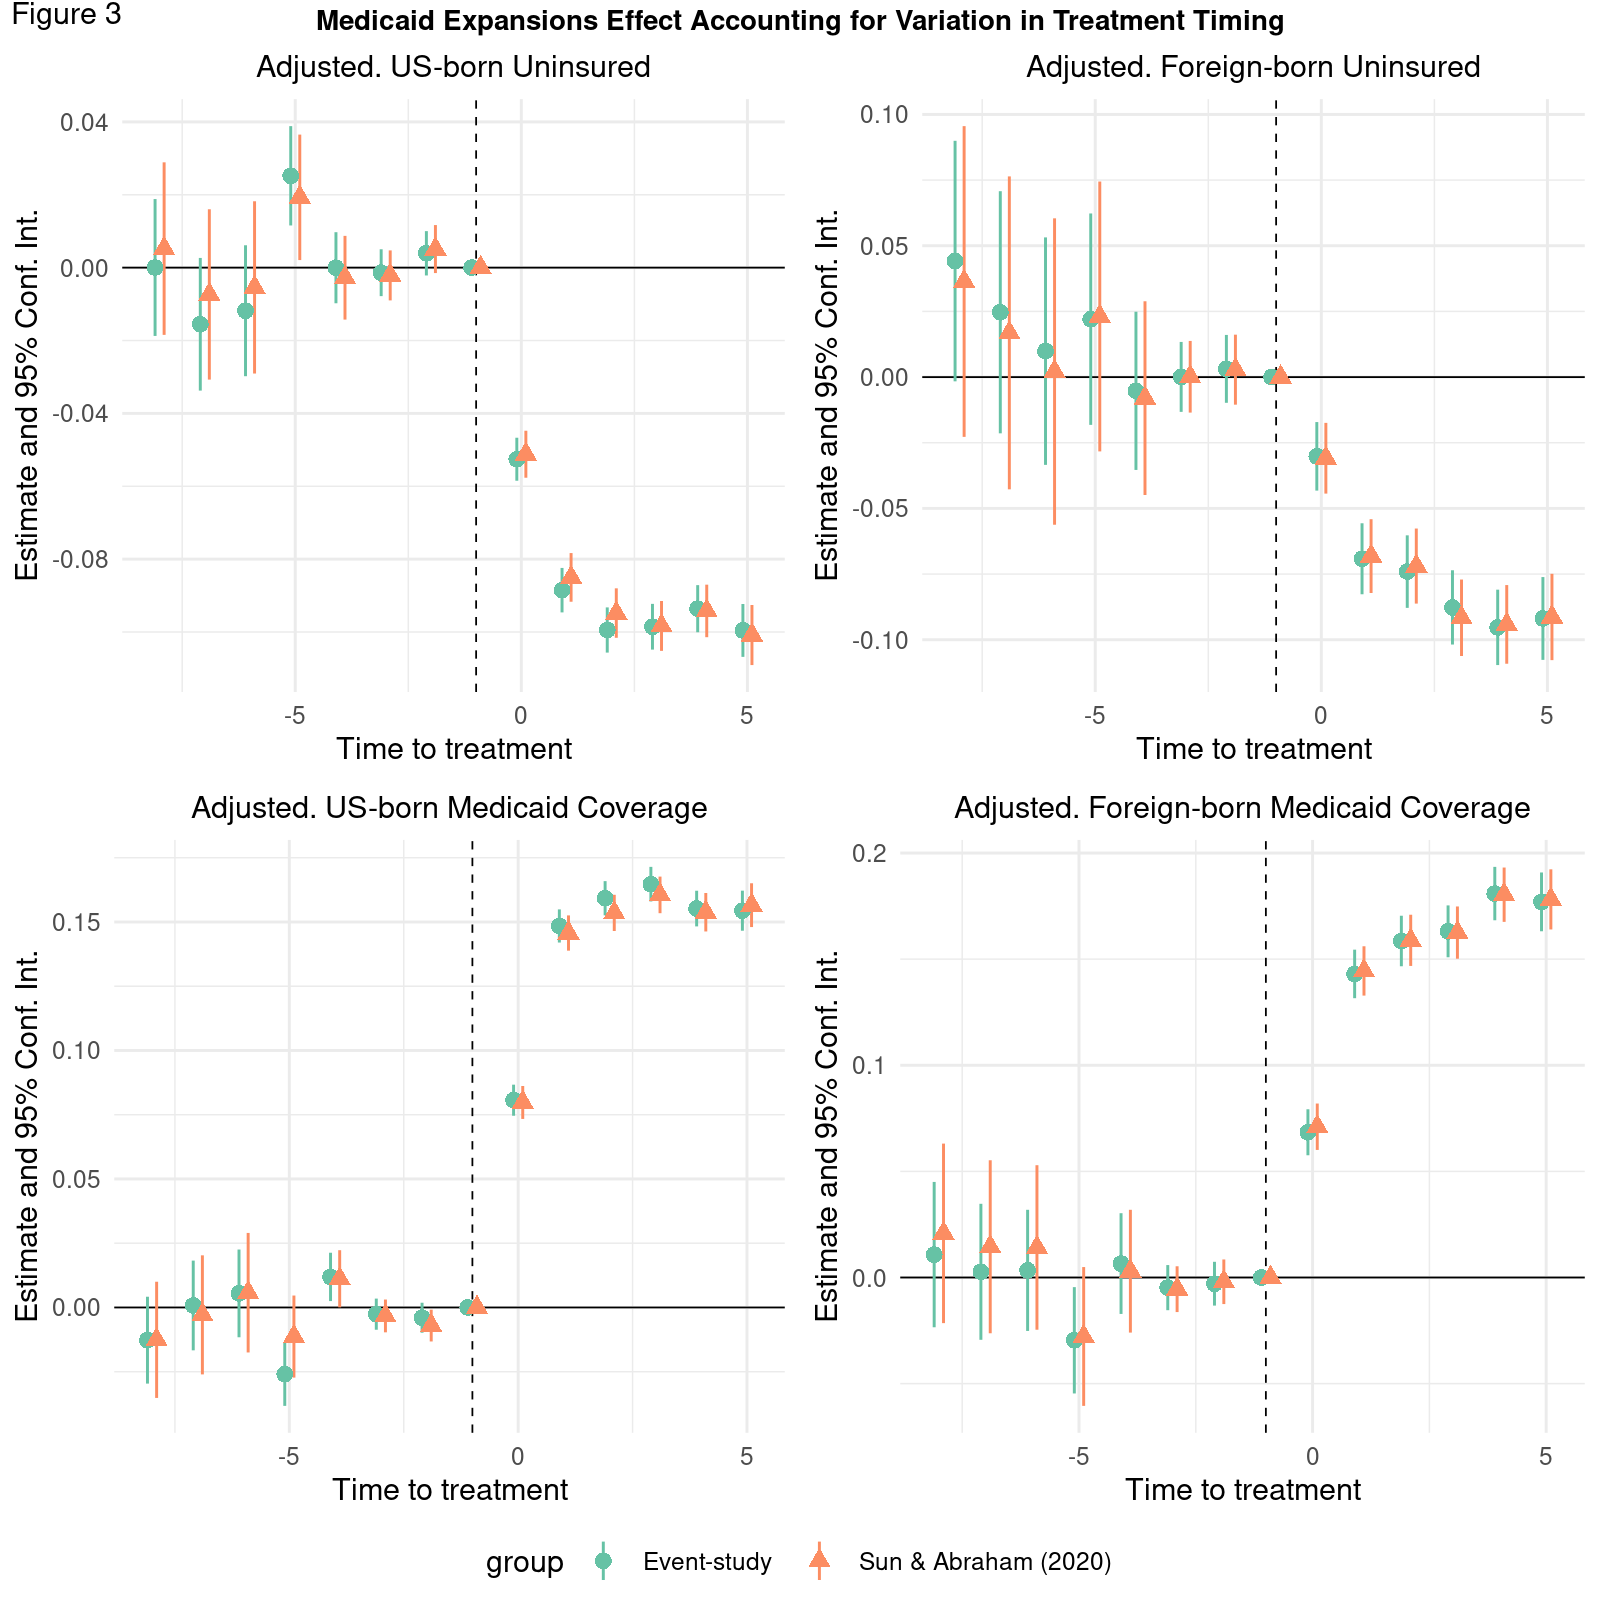
\includegraphics{~/Desktop/shadi/output/sun&abr-1} \end{center}

\hypertarget{difference-in-differences-estimate-bacon-decomposition-theorem}{%
\subsubsection{Difference-in-Differences Estimate: Bacon Decomposition
theorem}\label{difference-in-differences-estimate-bacon-decomposition-theorem}}

Employing Goodman-Bacon's (2018) methodology, we performed a
decomposition analysis utilizing two-way fixed effects
Difference-in-Differences (DID) estimators. This analysis provides
significant insights into the treatment effects and timing groups, as
outlined in Table 9.

\begin{table}

\caption{\label{tab:tab9}Bacon Decomposition}
\centering
\begin{tabular}[t]{lll}
\toprule
Comparison & Coefficient & Weight\\
\midrule
\addlinespace[1em]
\multicolumn{3}{l}{\textbf{Uninsured}}\\
\hspace{1em}Earlier vs Later Treated & -0.09309 & 0.11871\\
\hspace{1em}Later vs Earlier Treated & -0.05521 & 0.08771\\
\hspace{1em}Treated vs Untreated & -0.08462 & 0.79358\\
\addlinespace[0.3em]
\multicolumn{3}{l}{\textbf{Medicaid}}\\
\hspace{1em}Earlier vs Later Treated & 0.14610 & 0.11871\\
\hspace{1em}Later vs Earlier Treated & 0.08782 & 0.08771\\
\hspace{1em}Treated vs Untreated & 0.14452 & 0.79358\\
\bottomrule
\end{tabular}
\end{table}

The analysis involves comparing timing groups to units that never
received treatment, allowing us to evaluate the relative treatment
effects at different timings. Notably, a majority of the estimated
treatment effect can be attributed to the comparisons between treated
and untreated units, rather than comparisons between states with
different treatment times.

Furthermore, when we exclude the variation arising from comparisons of
states with different treatment times, the Difference-in-Differences
(DD) estimate remains highly consistent with the main DD estimate. In
simpler terms, the magnitude of the treatment effect produced by the
2014 wave is comparable to the effects observed in subsequent waves.
This robustness analysis strengthens our findings and affirms the
reliability of the estimated treatment effect.

\begin{center}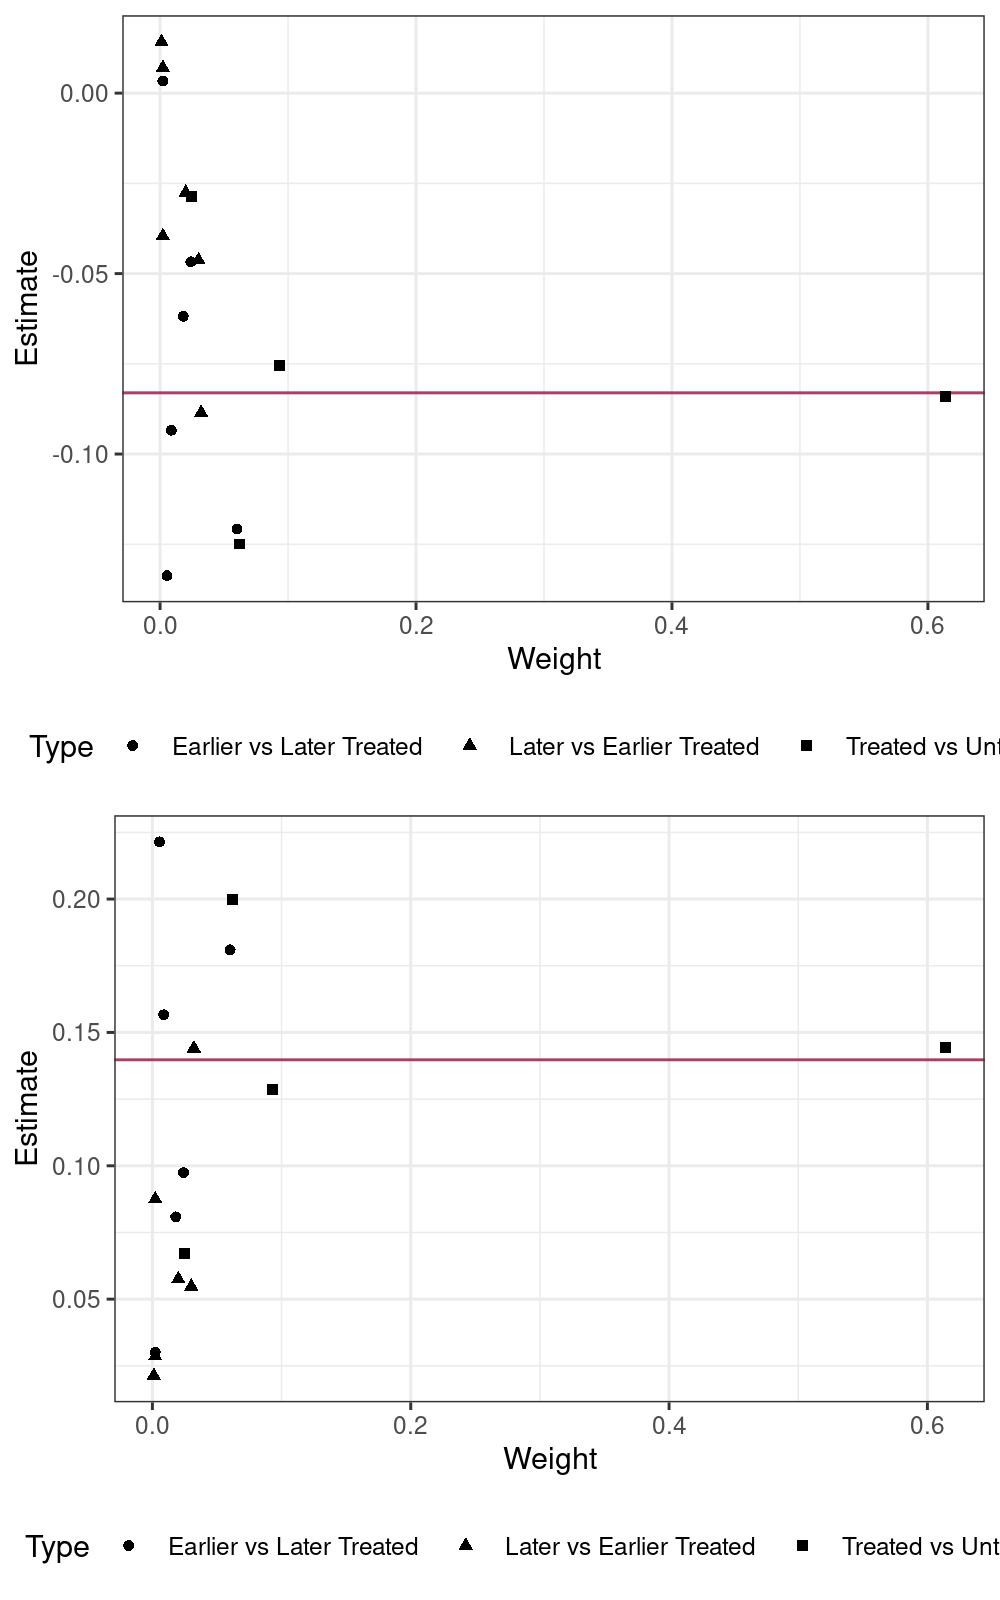
\includegraphics{~/Desktop/shadi/output/plotbac-1} \end{center}

Figure 4 provides support for this finding by presenting the 2 × 2 DD
estimates and associated weights derived from the conventional two-way
fixed effect model. Panel (a) illustrates the estimates for the
Uninsured group, while panel (b) exhibits the estimates for Medicaid
coverage.

\end{document}
